\documentclass[conference]{IEEEtran}
\IEEEoverridecommandlockouts
% The preceding line is only needed to identify funding in the first footnote. If that is unneeded, please comment it out.
\usepackage{cite}
\usepackage{amsmath,amssymb,amsfonts}
\usepackage{algorithmic}
\usepackage{graphicx}
\usepackage{textcomp}
\usepackage{xcolor}
\usepackage{subfigure}
\usepackage{multirow}

\begin{document}

\title{Random Selection of Parameters in Asynchronous Pool-Based Evolutionary Algorithms\\
}

\author{\IEEEauthorblockN{Mario Garc\'ia-Valdez, Ren\'e M\'arquez, Leonardo Trujillo}
  \IEEEauthorblockA{\textit{Instituto Tecnol\'ogico de Tijuana} \\
    mario@tectijuana.edu.mx}
  \and
  \IEEEauthorblockA{J.J. Merelo}
  \IEEEauthorblockN{Computer Architecture and Technology\\
    University of Granada, Spain\\
    jmerelo@ugr.es}
}

\maketitle
\begin{abstract}
  Synchronous operation is not the most natural setup in distributed
algorithms. In grid, cloud or volunteer setups nodes are
heterogeneous, or simply are not available at the exact same time;
this is a challenge for the researcher if their full performance is
going to be actually leveraged. Recently, in the field of Evolutionary
Algorithms (EAs), researchers have proposed several asynchronous 
designs have that distribute the evolutionary process among 
heterogeneous nodes. These algorithms share the population between distributed
workers which execute the actual evolutionary process by taking
samples of the population, and replacing them in the population pool
by evolved individuals. The performance of these EAs depends in part
on the selection of parameters for the EA running in each worker. In
this paper we study how varying randomly pararameters in distributed
evolutionary algorithms affect performance. Experiments 
were conducted in the AWS cloud using 2, 6 and 12
virtual machine configurations, with both homogeneous and
heterogeneous random settings using five test functions for
real-valued optimization (Rastrigin, Griewank, De Jong, Schaffer and
Ackley) and the OneMax binary problem. The results suggest that
this method can produce a performance that is competitive with 
instances of the algorithm using workers with parameters 
specially tuned for the benchmark.
\end{abstract}


\begin{IEEEkeywords}
  Distributed Evolutionary Algorithms, Volunteer Computing,
  Cloud Computing, pool-based evolutionary algorithms, parameter optimization. 
\end{IEEEkeywords}

\section{Introduction}

%Why Parallel
Biological evolution is a process with some interesting properties,
with which we can design computational systems, that are asynchronous,
parallel, and distributed;
however, it is not trivial to include some of these characteristics in standard
EAs, and many remain as sequential and synchronous algorithms \cite{eiben}.
A large body of work exists about the parallelization EAs, using multi-core, 
distributed systems, and GPUs \cite{cantu2000efficient,hofmann2013performance}.
However, only recently asynchronous and distributed EAs have started to become
a common practice, intending to exploit computing resources available everywhere
from personal computers, smartphones, and tablets, as well as data 
centers \cite{agajaj,FlexGP}. 

Access to these resources can be easily achived through popular Internet 
technologies, such as cloud computing, peer-to-peer (P2P), and web environments. 
Moreover, these technologies are intended for the
development of parallel, distributed and asynchronous systems, such
that an EA developed on top of them could easily reap the benefits of
these features.

%Pool Based
The focus of this work is on Pool-based EAs or PEAs, in which the search
is distributed to many processes that collaborate using a shared
repository or population pool. We highlight the fact that such
systems are intrinsically asynchronous, parallel, and distributed.
The particular PEA used in this paper is implemented on
the EvoSpace framework \cite{GValdez2015}
in which distributed nodes (or workers) asynchronously take a
sample of the population pool,  perform a local evolutionary search 
on it, and after several iterations, returns the sample contining 
newly evolved solutions.
% EA Paramaters
Like any other EA, the performance of the complete search procedure will depend
on the correct tuning of the parameters. However, settings
must be optimized to each particular problem \cite{de2007parameter}
giving users an additional optimization task.
Substantial work has focused on facilitating the burden of finding
the most appropriate parameters settings, suggesting several strategies:
using parameters of previous studies \cite{eiben1999parameter}
optimization by another genetic algorithm \cite{grefenstette1986optimization},
dynamic adaptation \cite{eiben1999parameter},
self-adaptive parameters \cite{pellerin2004self}, hybrid approaches \cite{de2007parameter} and so on.
% Worst on many workers
In heterogeneous and distributed PEAs like EvoSpace, this problem can
be magnified by a factor of $N$, the number of workers, because each one
can be treated as an independent EA with local parameters. Moreover, there
are additional parameters particular to the EvoSpace framework,
for instance the size of the samples.
% Dynamic adaptation
Several works propose the use of adaptive crossover and mutation probabilities
that depend on the current genetic diversity of the population \cite{pellerin2004self},
arguing that modifying these parameters can prevent the rapid convergence of the
algorithm.
% Explore and Exploit
% Is this pertinent?
A common dynamic heuristic is to explore the solution space first and then exploit
when a local optima is found and repeat if necessary.
% Random Patameters
Having multiple EAs running in parallel with different parameters could be
equivalent to performing a dynamic adaptation, having some workers exploring
and others exploiting at the same time.
% Evaluate in EvoSpace
In \cite{LNCS86720702} we introduced for the first time a method
inspired by the Randomized Parameter
Setting Strategy (RPSS) \cite{fuku1,fuku2}; in subsequent papers
\cite{hernandez2017randomized} we compared it with a dynamic
adaptation strategies, but applied to particle swarm optimization
algorithms.
In this paper, we apply it to EvoSpace and test on
several benchmark problems, extending the work presented in \cite{LNCS86720702}
in which only trap functions were considered.
The objective of RPSS is that, in a distributed EA, parametrization 
can be skipped entirely,With research showing that when the number of islands
is large enough, the algorithm parameters of each island can be randomly
set and still achieving good results overall. However, most of the work on 
RPSS has been in the well-known Island Model for EAs, 
a distributed but synchronous system. In this paper we will apply 
it to asynchronous EAs implemented using a pool-based strategy.

The paper organization is as follows. In Section \ref{sec:work} we
review the related work. Afterwards,in Section \ref{sec:evo} we briefly describe the
proposed EvoSpace cloud implementation, the experimental work is next in
Section \ref{sec:experiments}. Finally, we give summary and concluding remarks in
Section \ref{sec:conclusions}.

\section{Related Work}
\label{sec:work}

The number of parameters that need to be tuned and the computational cost of
exploring an ample search space are two common issues faced by designers of
EAs.  Regarding the computational cost, a common approach to mitigate the
problem is to follow a parallel or a distributed design \cite{cantu-paz:migration-policies,duda2013gpu}.
For instance, Fern\'andez et al. \cite{nc} 
uses the well-known Berkeley Open Infrastructure for Network Computing (BOINC) to distribute EA runs across a
heterogeneous network of volunteer computers using virtual machines. Another  example is
found in the FlexGP system developed by Sherry et al. \cite{FlexGP}. FlexGP is probably the first large scale GP system
that runs on the cloud, using an Island model approach and implemented over Amazon EC2 with a
socket-based client-server architecture. Even recently, this client-server architecture has been used profitably by researchers such as Salza and Ferrucci \cite{SALZA2019276} for speeding up evolutionary algorithms in a cloud infrastructure. Lately, implementations tend to use Docker containers instead of virtual machines \cite{Dziurzanski2020}.

Distributed evolutionary algorithms using client-server implementations are a good match for fixed infrastructure, such as clusters, supercomputers or simply multi-core architectures, and they continue to be researched actively \cite{Liu201954}, but another approach to distributed EAs is the so called pool-based architecture \cite{sofea:naco}. In general, a
pool-based system employs a central repository where (maybe a part of) the evolving population is stored.
Distributed clients interact with the pool, performing some or all of the basic EA processes
(selection, genetic operators, survival). An initial work implementing this approach (and without calling it by tha name)
is that by Merelo et al. \cite{agajaj} implementing a JavaScript based PEA that distributes
the evolutionary process over the web, providing the added advantage of not requiring the
installation of additional software in each computing node; a similar approach which uses a blockchain-like data store called FluidInfo \cite{radcliffe2012getting} was also proposed by the same authors in \cite{DBLP:conf/cec/Merelo10}.  Other similar cloud-based solutions
are based on a global queue of tasks and a Map-Reduce implementation which normally handles failures
by the re-submission of  tasks \cite{fazenda2012,di2013towards,FlexGP}. This work was initiated by distributing tasks using the BOINC
volunteer platform;  Smaoui et al. \cite{FekiNG09} uses work units that consist of a fitness
evaluation task and multiple replicas  were produced and sent to different clients.

While using a distributed framework can ease the computational cost, it can also exacerbate the first issue mentioned above;
i.e., it increases the size of the algorithm parameter space, which makes parameter tuning a more difficult task.
The issue of optimal parametrization of EAs has been  widely studied \cite{de2007parameter},
with many approaches in literature. For instance, one of the most successful approaches
is the F-Racing and iterative F-Racing techniques \cite{lopez2011irace}; these use optimization techniques to explore the parameter space; parameter setting can also be approached theoretically, at least in a class of optimization problems, as proved by Doerr et al. in \cite{doerr2020theory}. However, this implies that either you need to run a meta-algorithm in order to find an efficient parametrization, or try to look for a theoretical approach to the specific problem that is able to give you a good parametrization. 

In this paper, we will take a lateral approach to this problem, inspired by the approach proposed by Gong and Fukunaga
called RPSS \cite{fuku1,fuku2}.
Originally proposed for an Island Model EA, RPSS sets the parameter values of each subpopulation randomly,
without any kind of tuning or self-adaptive process. The RPSS approach is to set the parameters
of each subpopulation randomly at the beginning of the run, a very simple strategy.
Even so, results reported in \cite{fuku1,fuku2} exhibit promise, achieving competitive results
while substantially reducing the amount of effort required to tune the system.

In a first study, \cite{LNCS86720702} reported that in effect RPSS
can be successfully applied to a PEA. However, in that work the
approach was only tested on the P-Peaks generator of multi-modal problems proposed by De Jong et al. \cite{Jong:PS97}.
While the problem is theoretically interesting, it can be limited in scope given its reliance on a bit string representation.
Therefore, this work extends the study considering another binary representation problem (OneMax) as well as
five high-dimensional real-valued optimization benchmarks. Our goal is
to test how general is this approach by considering different search
spaces and different forms of fitness landscapes.

\begin{figure*}[h!tbp]
    \centering
        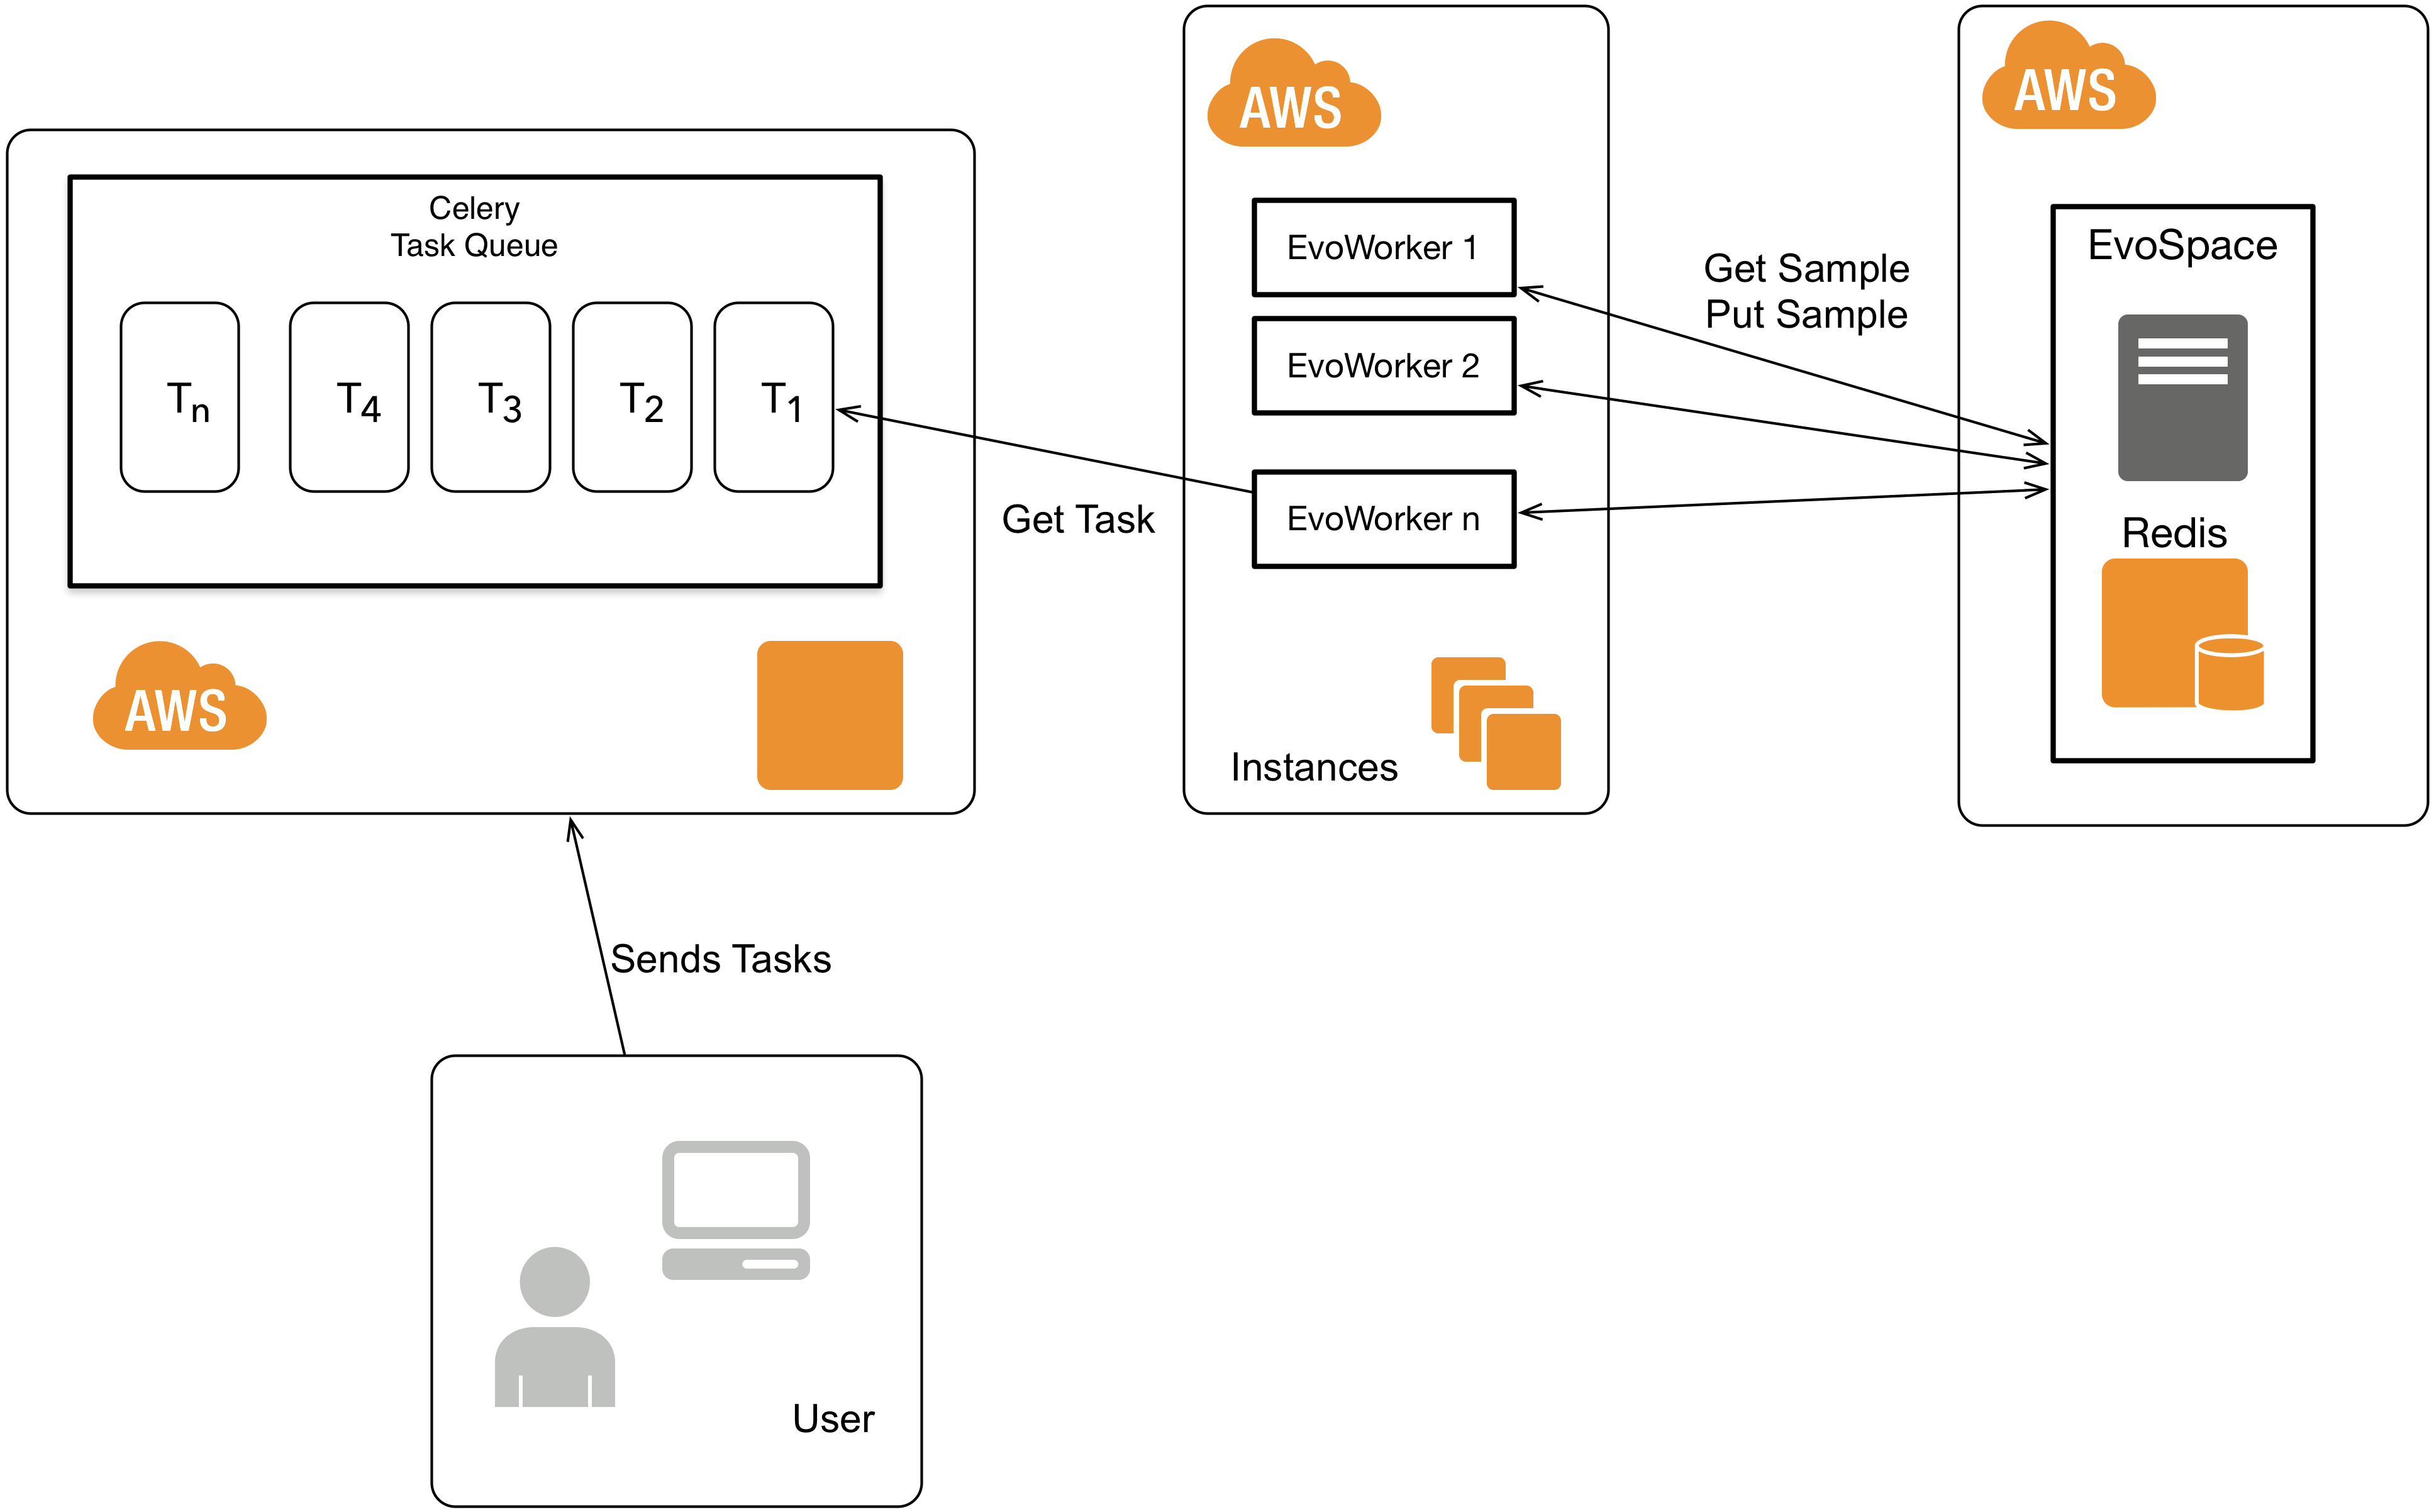
\includegraphics[width=10cm]{img/EvoSpaceAWS.png}
    \caption{Main components and data-flow in the cloud version of EvoSpace we are using in this paper.}
    \label{fig:evospace}
  \end{figure*}
%
\section{EvoSpace Cloud Implementation}
\label{sec:evo}

The EvoSpace framework, which was introduced in \cite{Evospace}, and
since then used in several applications \cite{GValdez2015} has two components: (i) the EvoSpace
container that stores the evolving population; and (ii) workers, which execute
the actual evolutionary process, while the EvoSpace container acts only as a population repository.
In a basic configuration, workers pull a small random sample of the
population, and use it as the initial population for a local EA executed
on the client machine. Afterward, the evolved population from each worker
is returned to the EvoSpace container. The experimental platform used in this work is
described in \cite{valenzuela2015implementing}, and consists of several virtual machines
created automatically by a script before each experiment. The main components are depicted
in Figure \ref{fig:evospace}. Each experiment consists of the following steps:

\begin{enumerate}
    \item First, the script creates two virtual machines: one for the task queue and another
    for the EvoSpace container. Then it creates the number of worker machines needed, these
    machines are configured as client machines for the task queue.
    \item For each run the number of EvoWorkers needed are added to the queue as tasks, from
    the user's PC.
    \item Every worker machine loads the task and the experiment
      starts. During the experiment every worker takes from and replaces
      samples in the EvoSpace container.
    \item Finally, all the data generated in each workers is returned by the task queue.
    \end{enumerate}

This setup was deployed on top of the Amazon Web Services (AWS)
platform which allowed the execution of the experiments with similar computing resources.
% Architecture Components
% Random Patameters

\section{Experiments}
 \label{sec:experiments}

\begin{table}[!t]
\caption{Valid ranges for each EvoWorker parameters. One Max}
\label{tab:params}
\centering
\begin{tabular}{|l|c|c|c|c|c|c| }
\hline
\textbf{Parameter} & \multicolumn{3}{|c|}{OneMax} & \multicolumn{3}{|c|}{Test Functions} \\
\hline
Number of Workers & 2 & 6 & 12 & 2 & 6 & 12\\
\hline
\hline
Population Size & 200 & 280 & 620 & 120 & 150 & 150\\
\hline
Sample Size & 40 & 40 & 40 & 40 & 20 & 10\\
\hline
Maximum Samples & 30 & 40 & 40 & 200 & 100 & 50\\
\hline
Local Generations & 30 & 30 & 30 & 100 & 100 & 100\\
\hline
\end{tabular}
\end{table}
%
The goal of this work is to determine if a random static parametrization for each of the $n$ EvoWorkers
collaborating on a given run could achieve competitive results against an homogeneous tuned parametrization
\cite{fuku1,fuku2,LNCS86720702}. The parameters considered to be randomly set for each EvoWorker
where the crossover and mutation probabilities with a valid range of $[0,1]$. These parameters where
selected because they effectively control which types of moves in the search space are
applied, and are related to the amount of exploration and exploitation
that is carried out. % \cite{}. Don't know if we need this - JJ
The other parameters and design choices used by EvoSpace and the EvoWorkers in our experiments are given in
Table \ref{tab:params}. Additionally, for the binary OneMax problem bit-flip mutation
is used with an independent probability for each attribute to be flipped (indpb) of $0.05$,
a two point crossover and a tournament selection of size 3. For the real-valued problems a Gaussian
mutation was applied with mu=$0$, sigma=$0.2$, and indpb=$0.05$; two point crossover and
a tournament selection of three. These values are kept static to measure only the effect of the
parameters mentioned above.


To measure the effectiveness of RPSS in EvoSpace two parametrization strategies are compared,
similar to what is done in \cite{fuku1,fuku2,LNCS86720702}. First, we consider the approach of setting all
of the EvoWorker parameters homogeneously. In order to tune the homogeneous parameters,
we select the best configuration from 100 random parametrizations.
Each of these random parametrization are evaluated based on their average performance over 10
independent runs for each problem.
Hereafter, we refer to this method as the {\em homogeneous} configuration.
Second, for RPSS the parametrizations
are not tuned, they are randomly generated for each EvoWorker, set independently at the beginning of each run.
Hereafter, we call this approach the {\em heterogeneous} configuration. Finally, we perform 30 independent runs
with both methods and report the average number of evaluations required by each strategy to find the
global optimum solution.

% I have moved this here to rearrange a bit graphics. This pushed down the whole thing.
\begin{figure*}[h!tb]
    \centering
    \subfigure [2 workers]
    {
        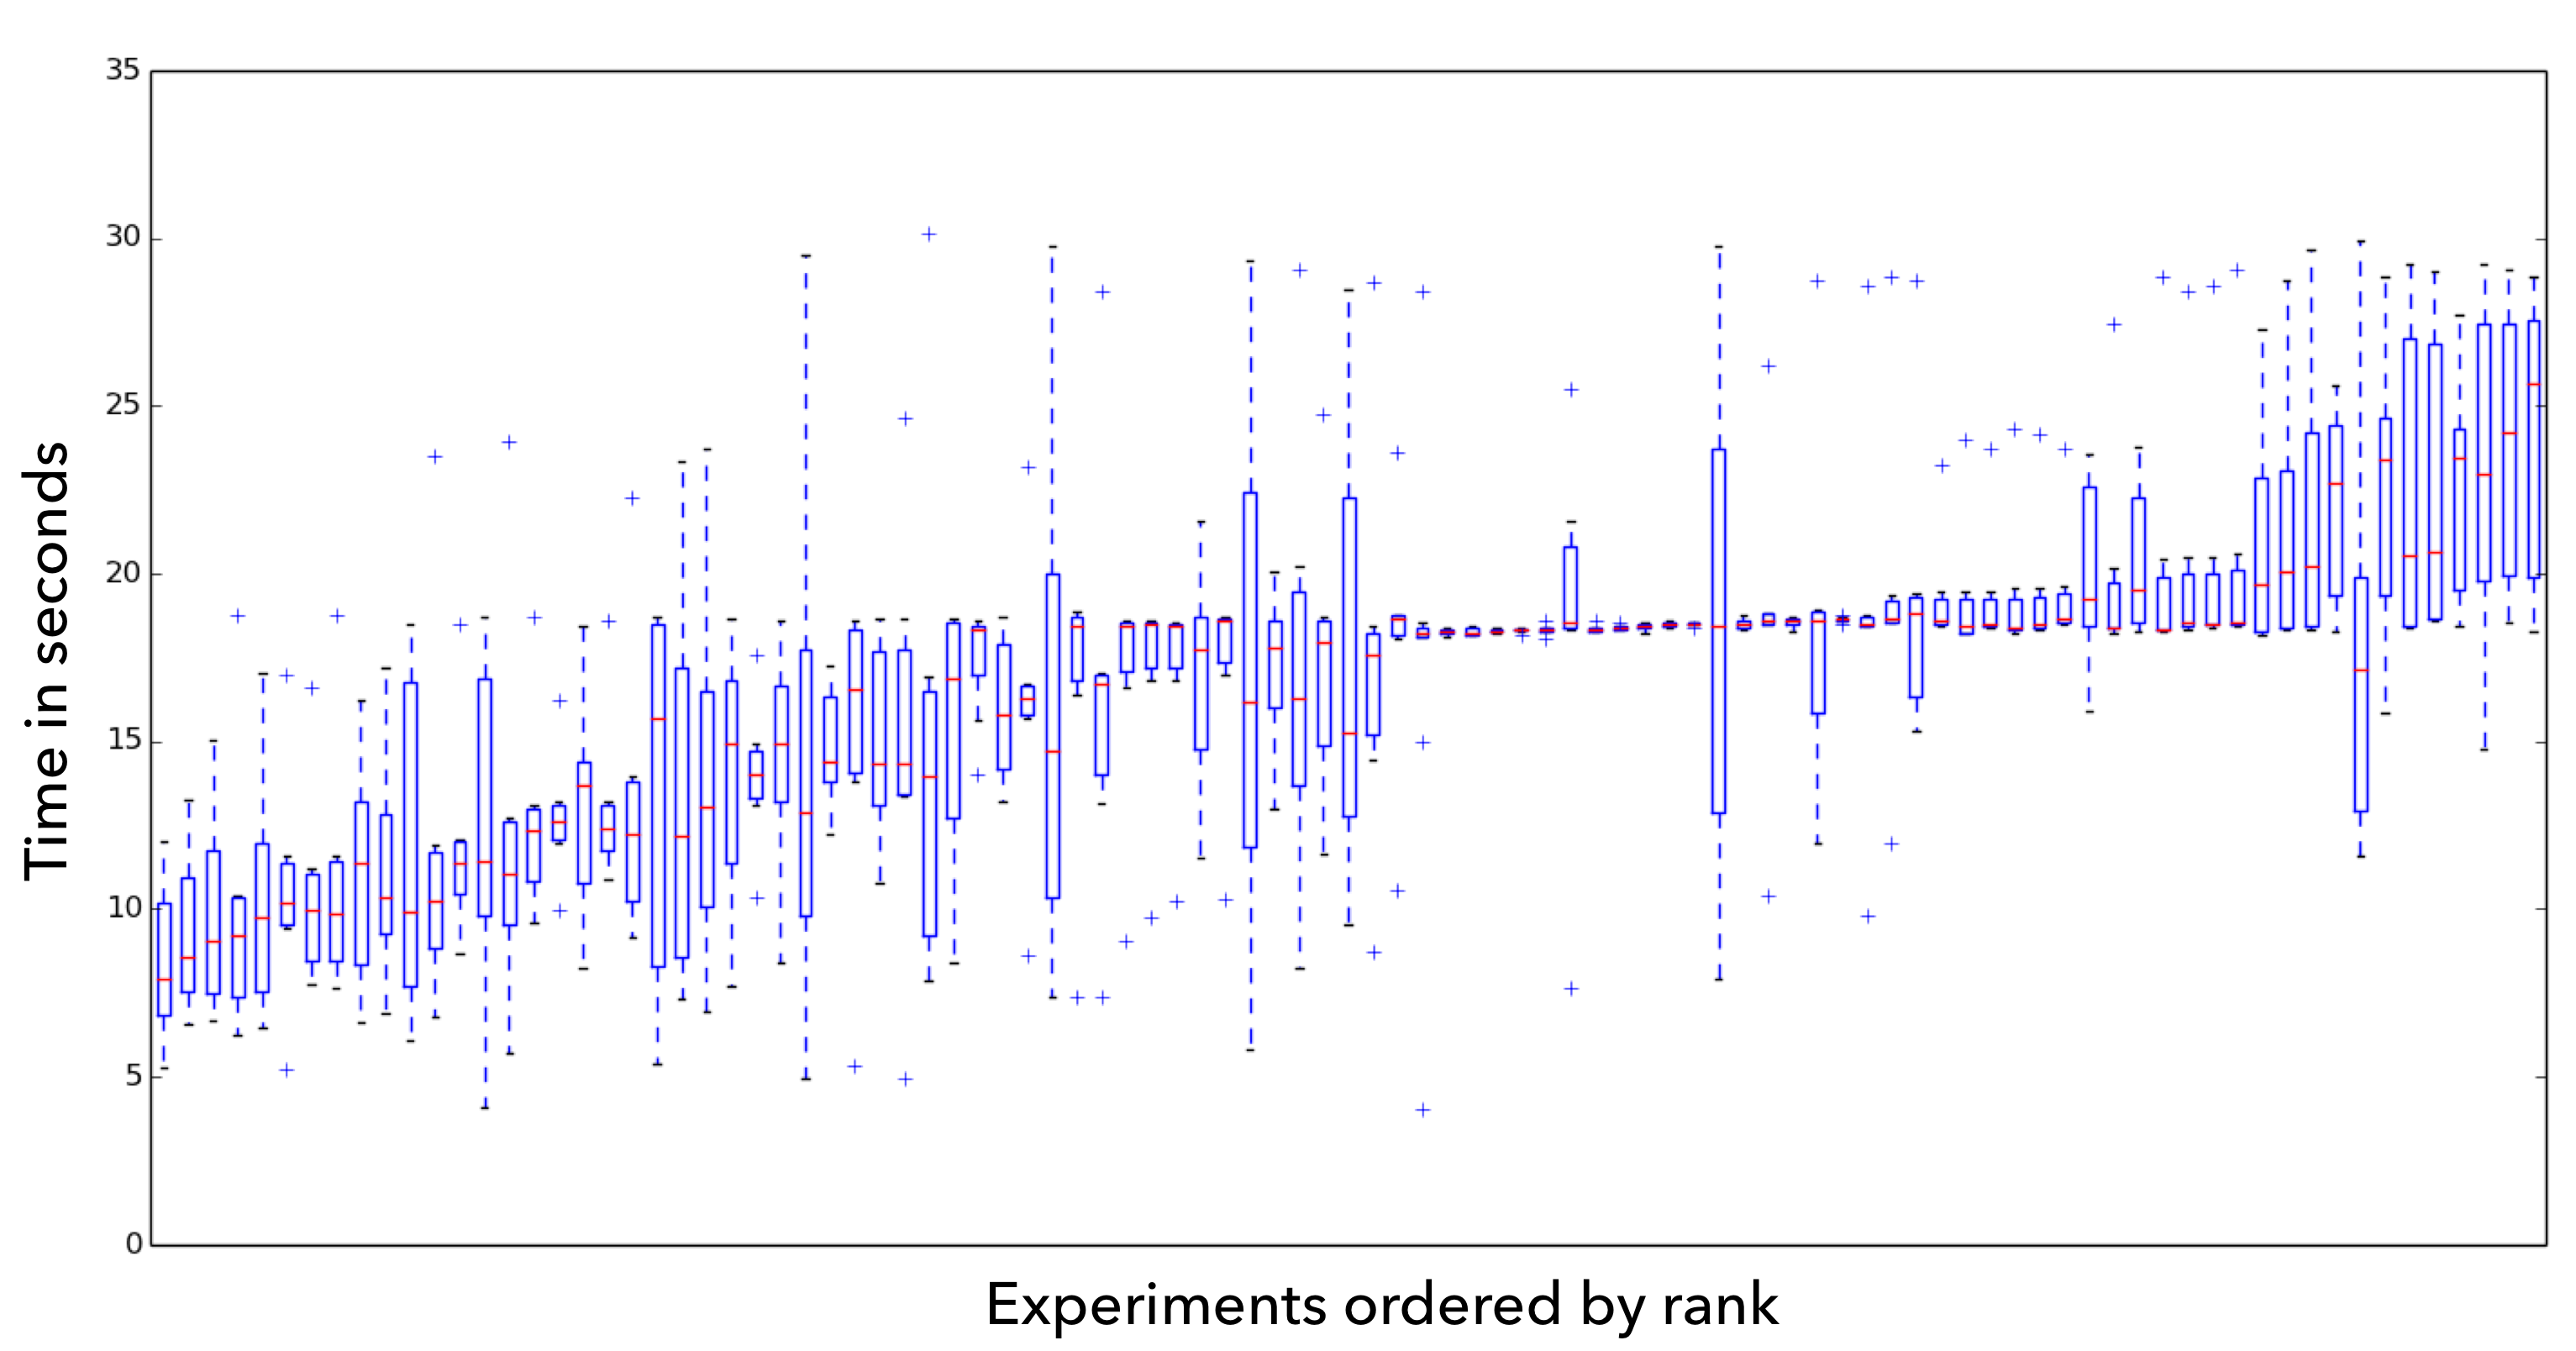
\includegraphics[width=4in]{img/2w_onemax_100_box.png}
    }
    \subfigure  [6 workers]
    {
        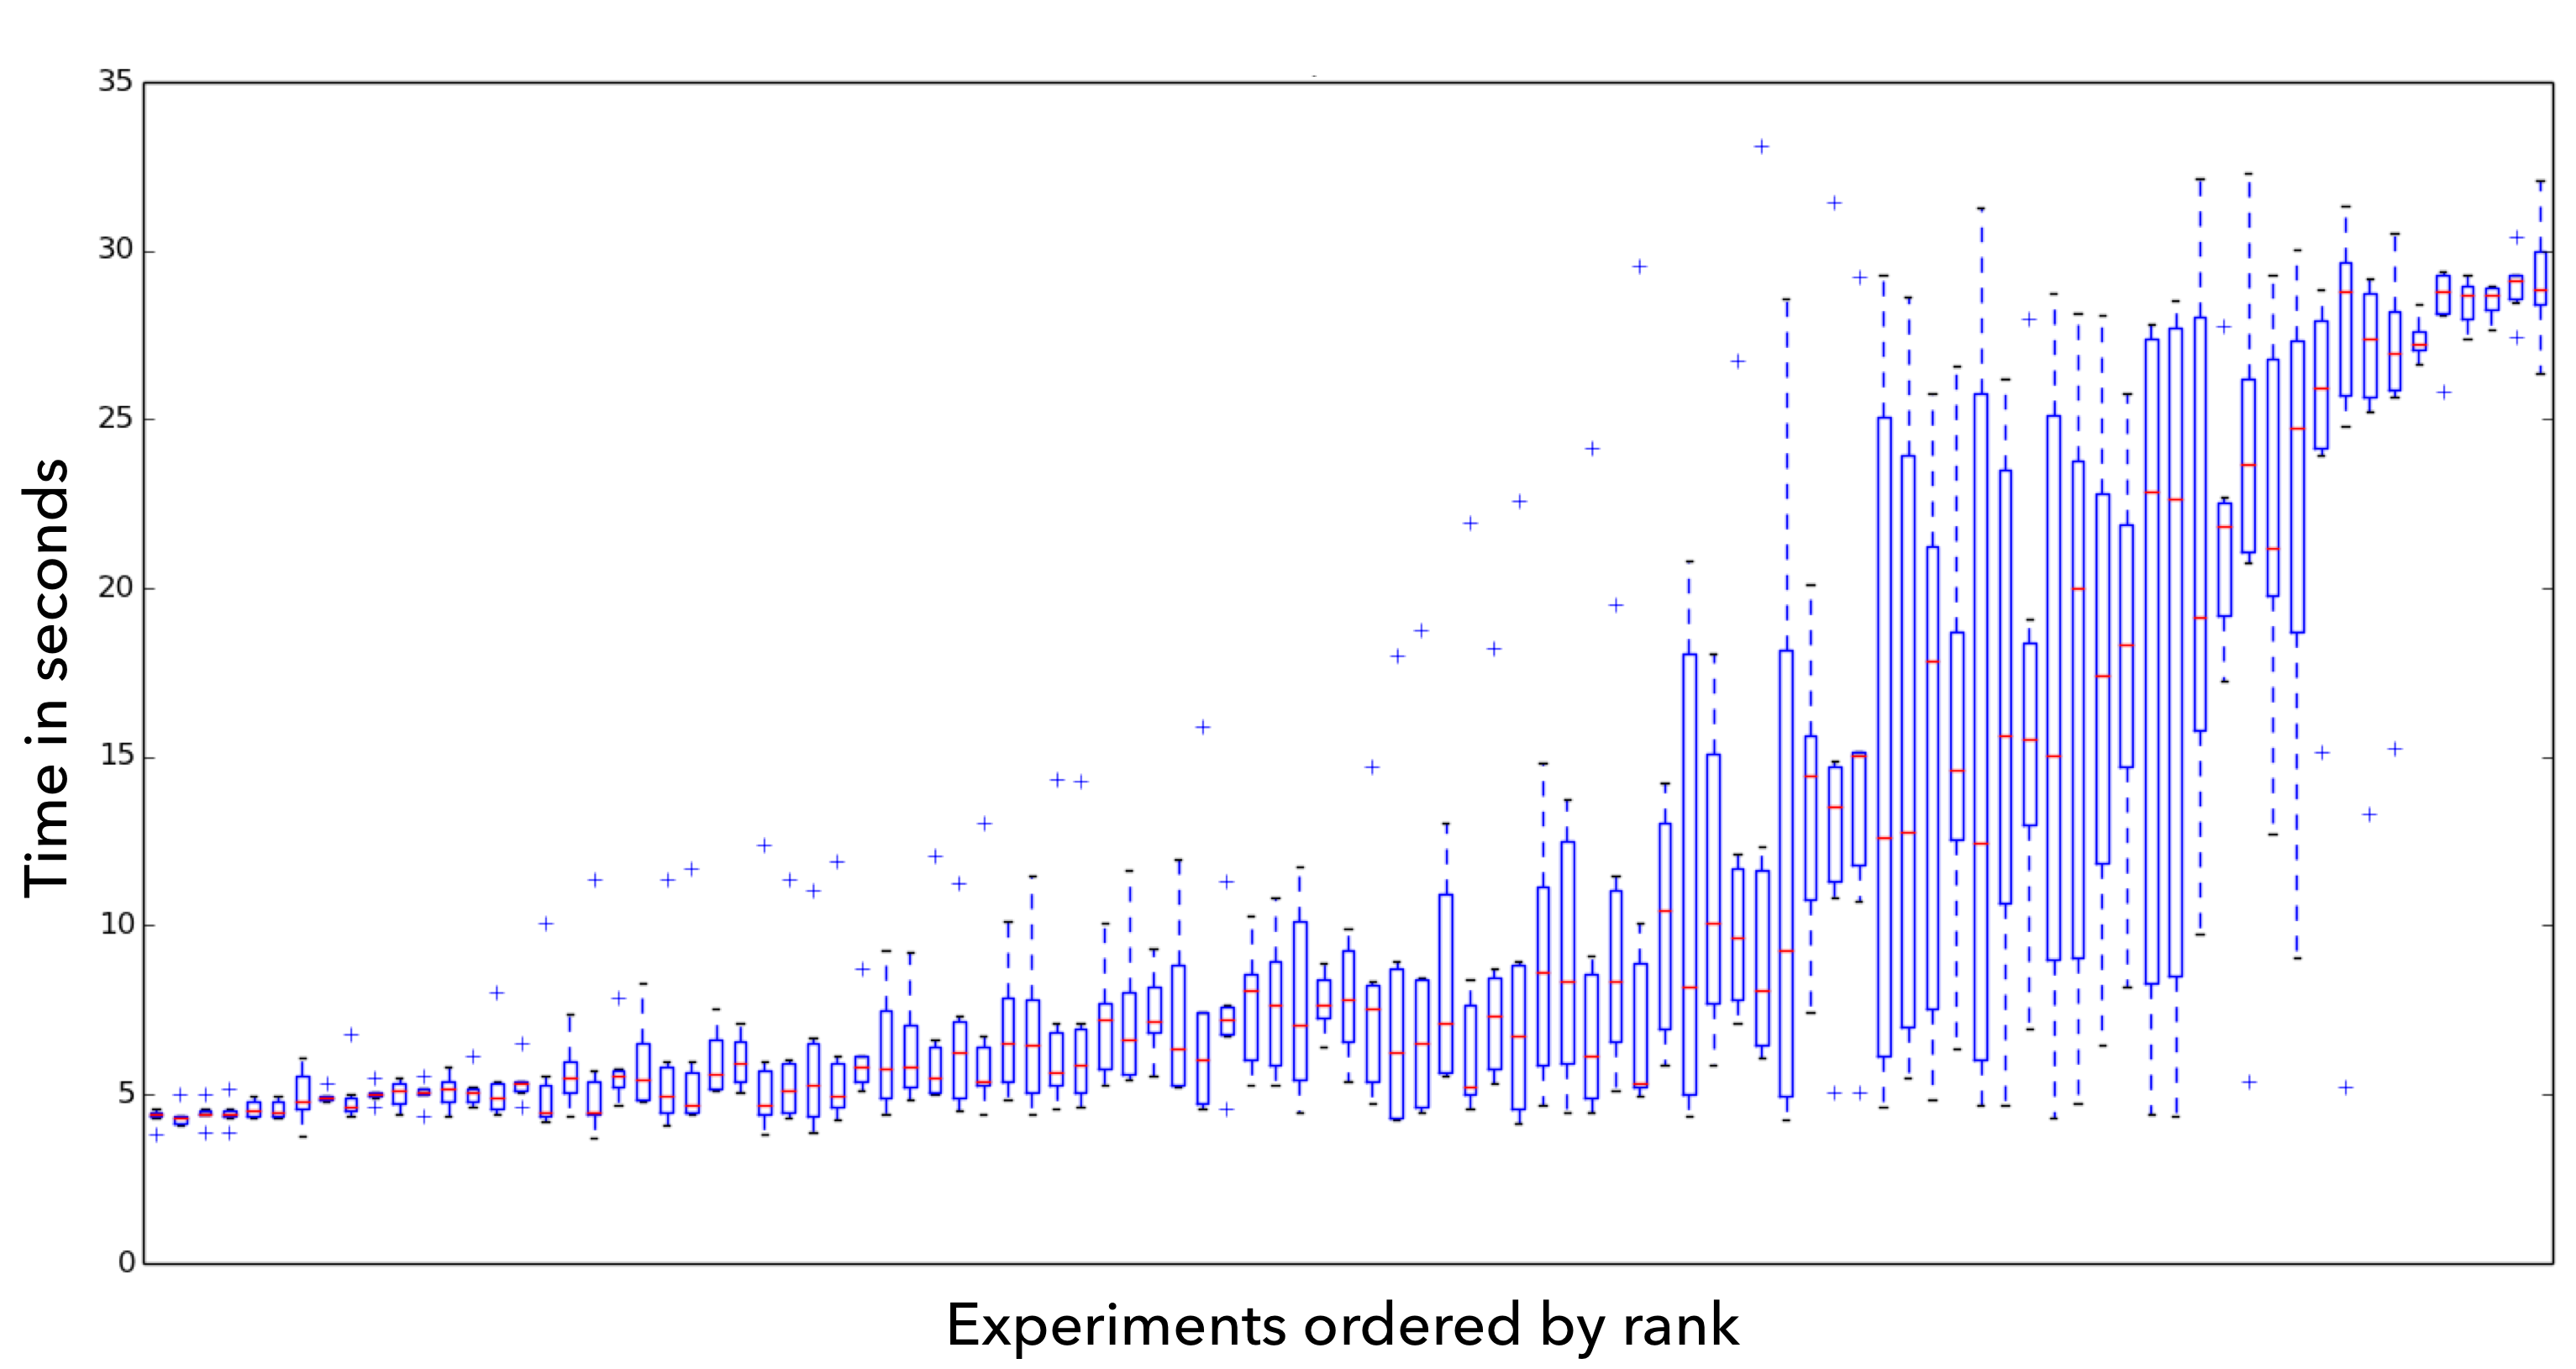
\includegraphics[width=4in]{img/6w_onemax_100_box.png}
    }
    \subfigure  [12 workers]
    {
        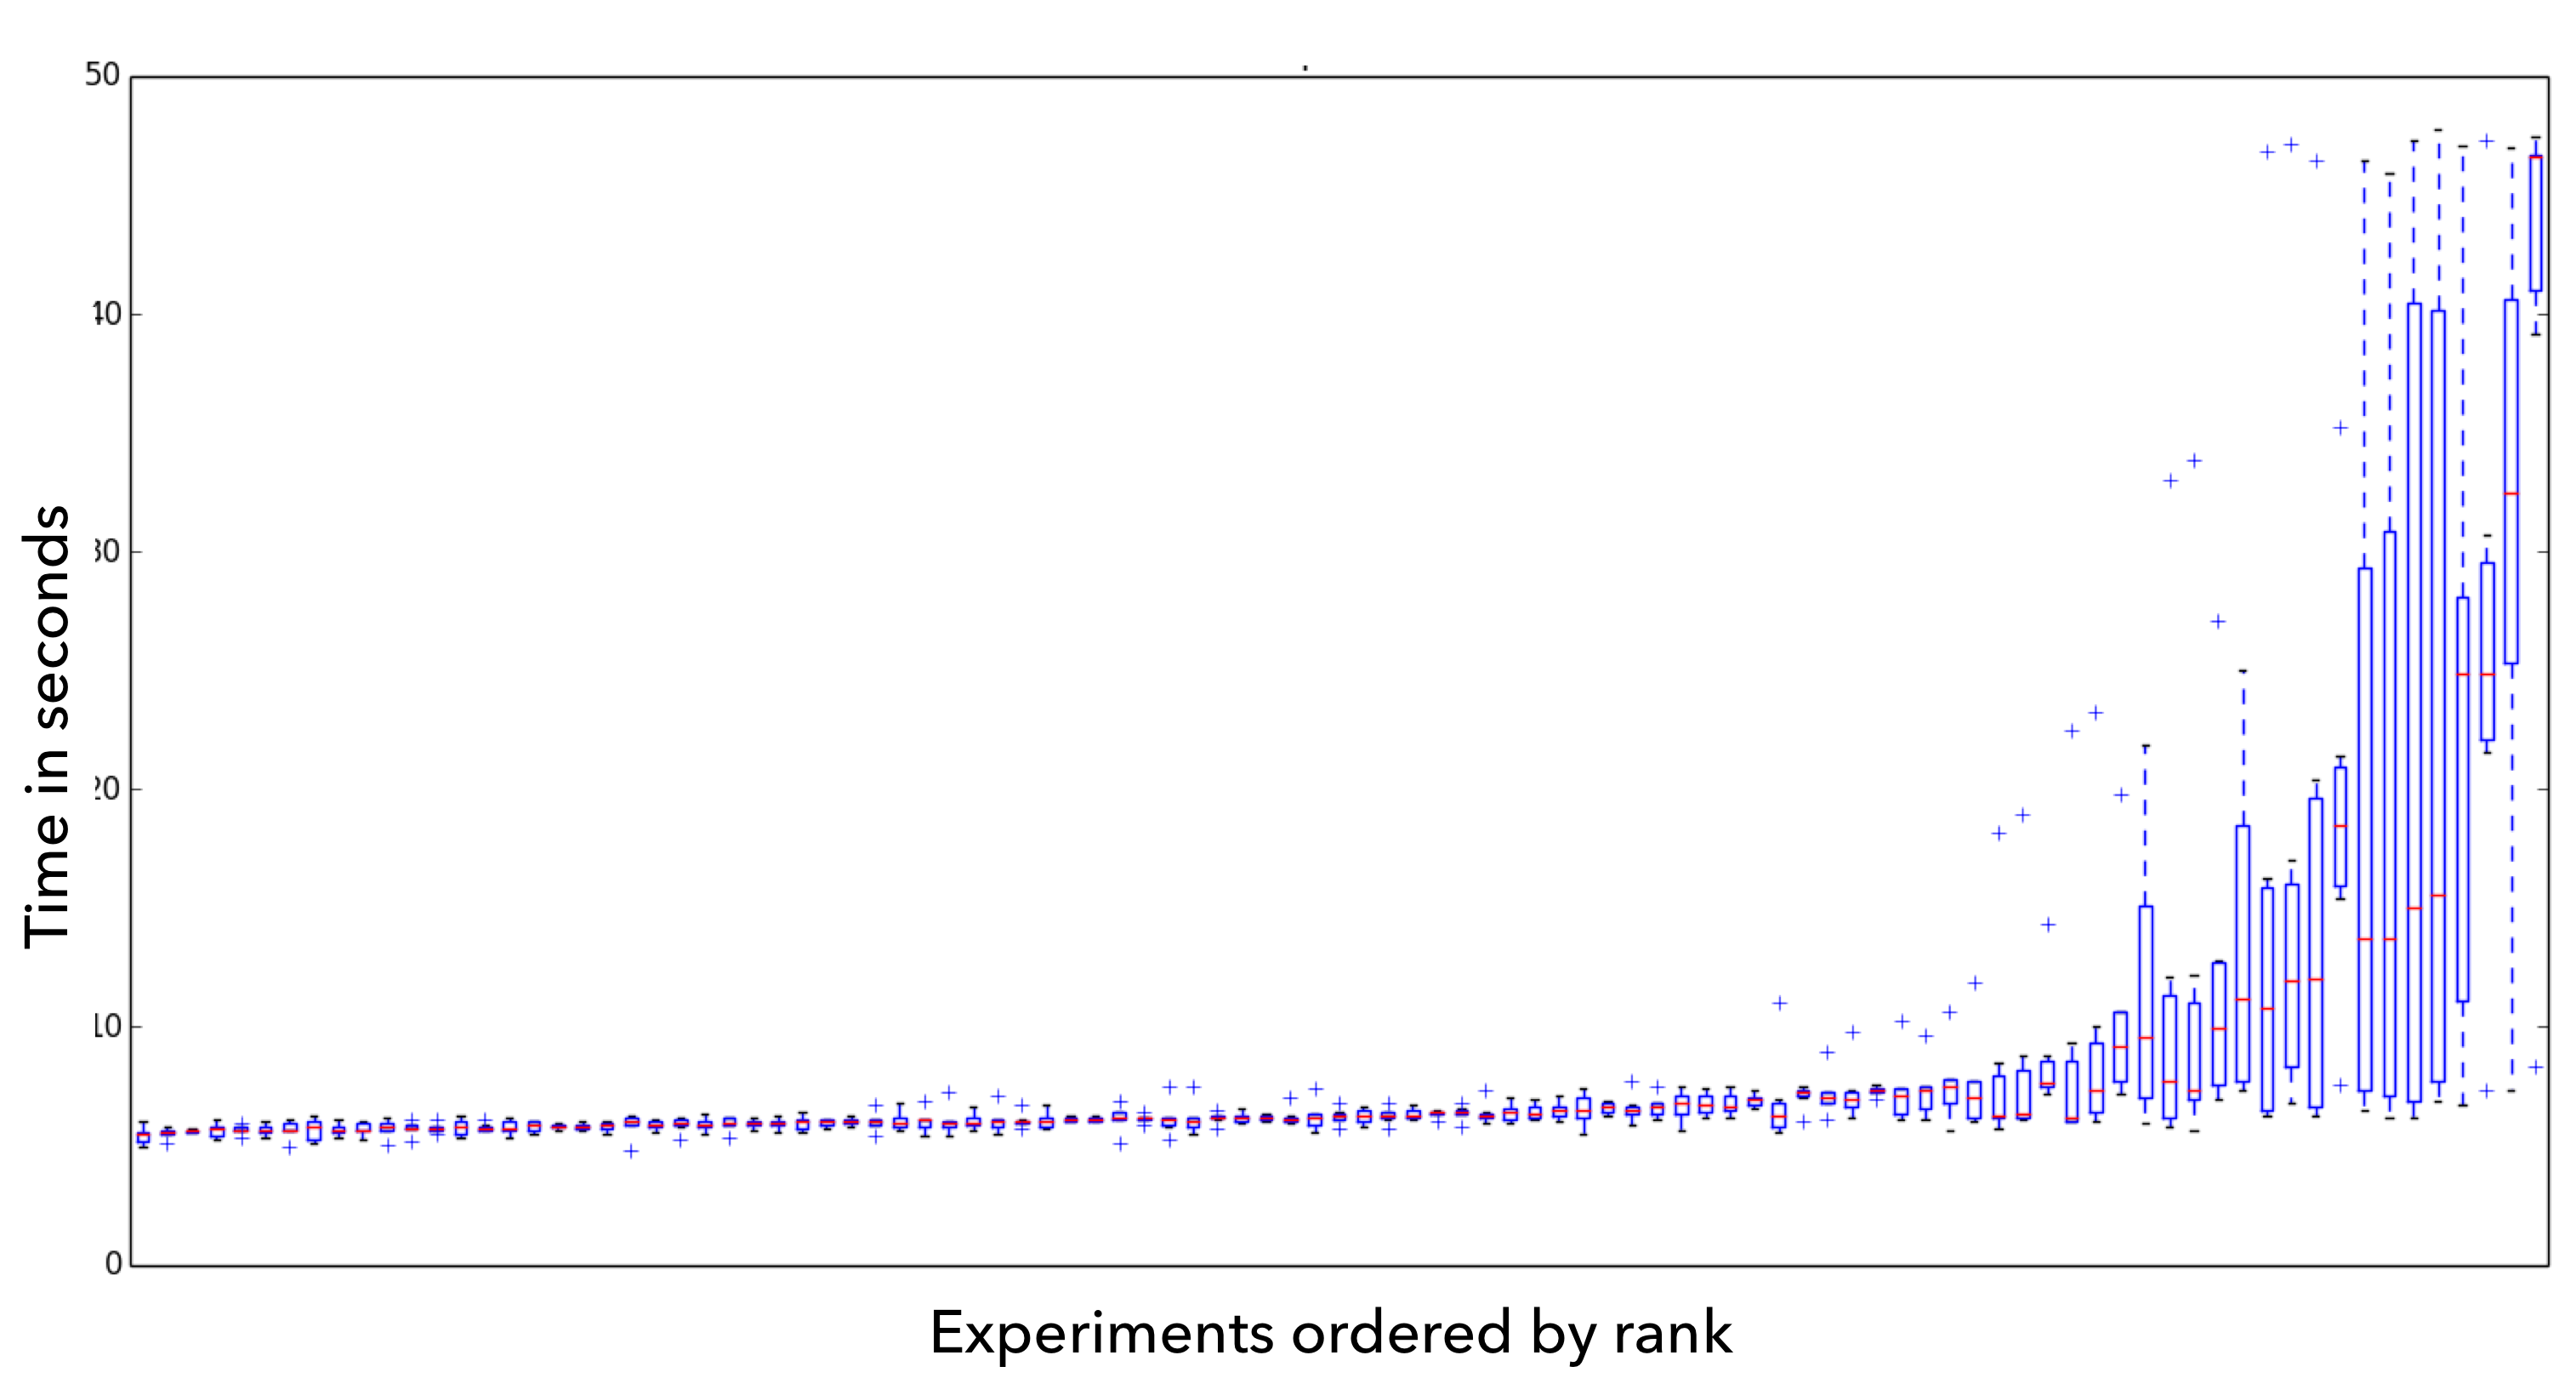
\includegraphics[width=4in]{img/12w_onemax_100_box.png}
    }

    \caption{100 experiments with random parameters for the 128 Bit OneMax problem.
    Experiments are ranked in increasing order by the average time to solution in 5 runs, with
    (a) 2 workers, (b) 6 workers, and (c) 12 workers.}
    \label{fig:effort}
  \end{figure*}
  %
The algorithms are first evaluated using the OneMax (or BitCounting) problem proposed by
Schaffer and Eshelman \cite{SE91}, this is a simple problem consisting in maximizing the number
of ones of a bitstring. Although the OneMax problem may not justify the use of a distributed
implementation, i.e. we can argue that it can be solved in a very short time by using a
single desktop computer, but on the other hand, it offers several advantages as a
benchmark for new architectures. It is a well-known problem with several
studies on parameters,  runtime analyses \cite{DBLP:journals/corr/MereloGVB15},
and distributed implementation
issues. On the other hand, the drawback of using a benchmark that is not representative of
real-world problems is that experimental results may be only applicable to
problems similar to OneMax, where genetic operators are well suited for the
search in a solution space without deceptive or very large landscapes.
For the current experiments a 128 bit string was used. Since this
problem is not computationally demanding, more experiments where conducted for the tuning phase,
tuning the parameters using 2, 6, and 12 EvoWorkers. Then, following \cite{fuku1},
five standard real-valued single objective optimization problems
are used, these are the Rastrigin, Griewank, De Jong, Schaffer  and Ackley functions,
with the number of dimensions set to 100 in each case. For these problems we use a real-valued vector
representation for each individual.

  \begin{figure*}[h!tb]
    \centering
        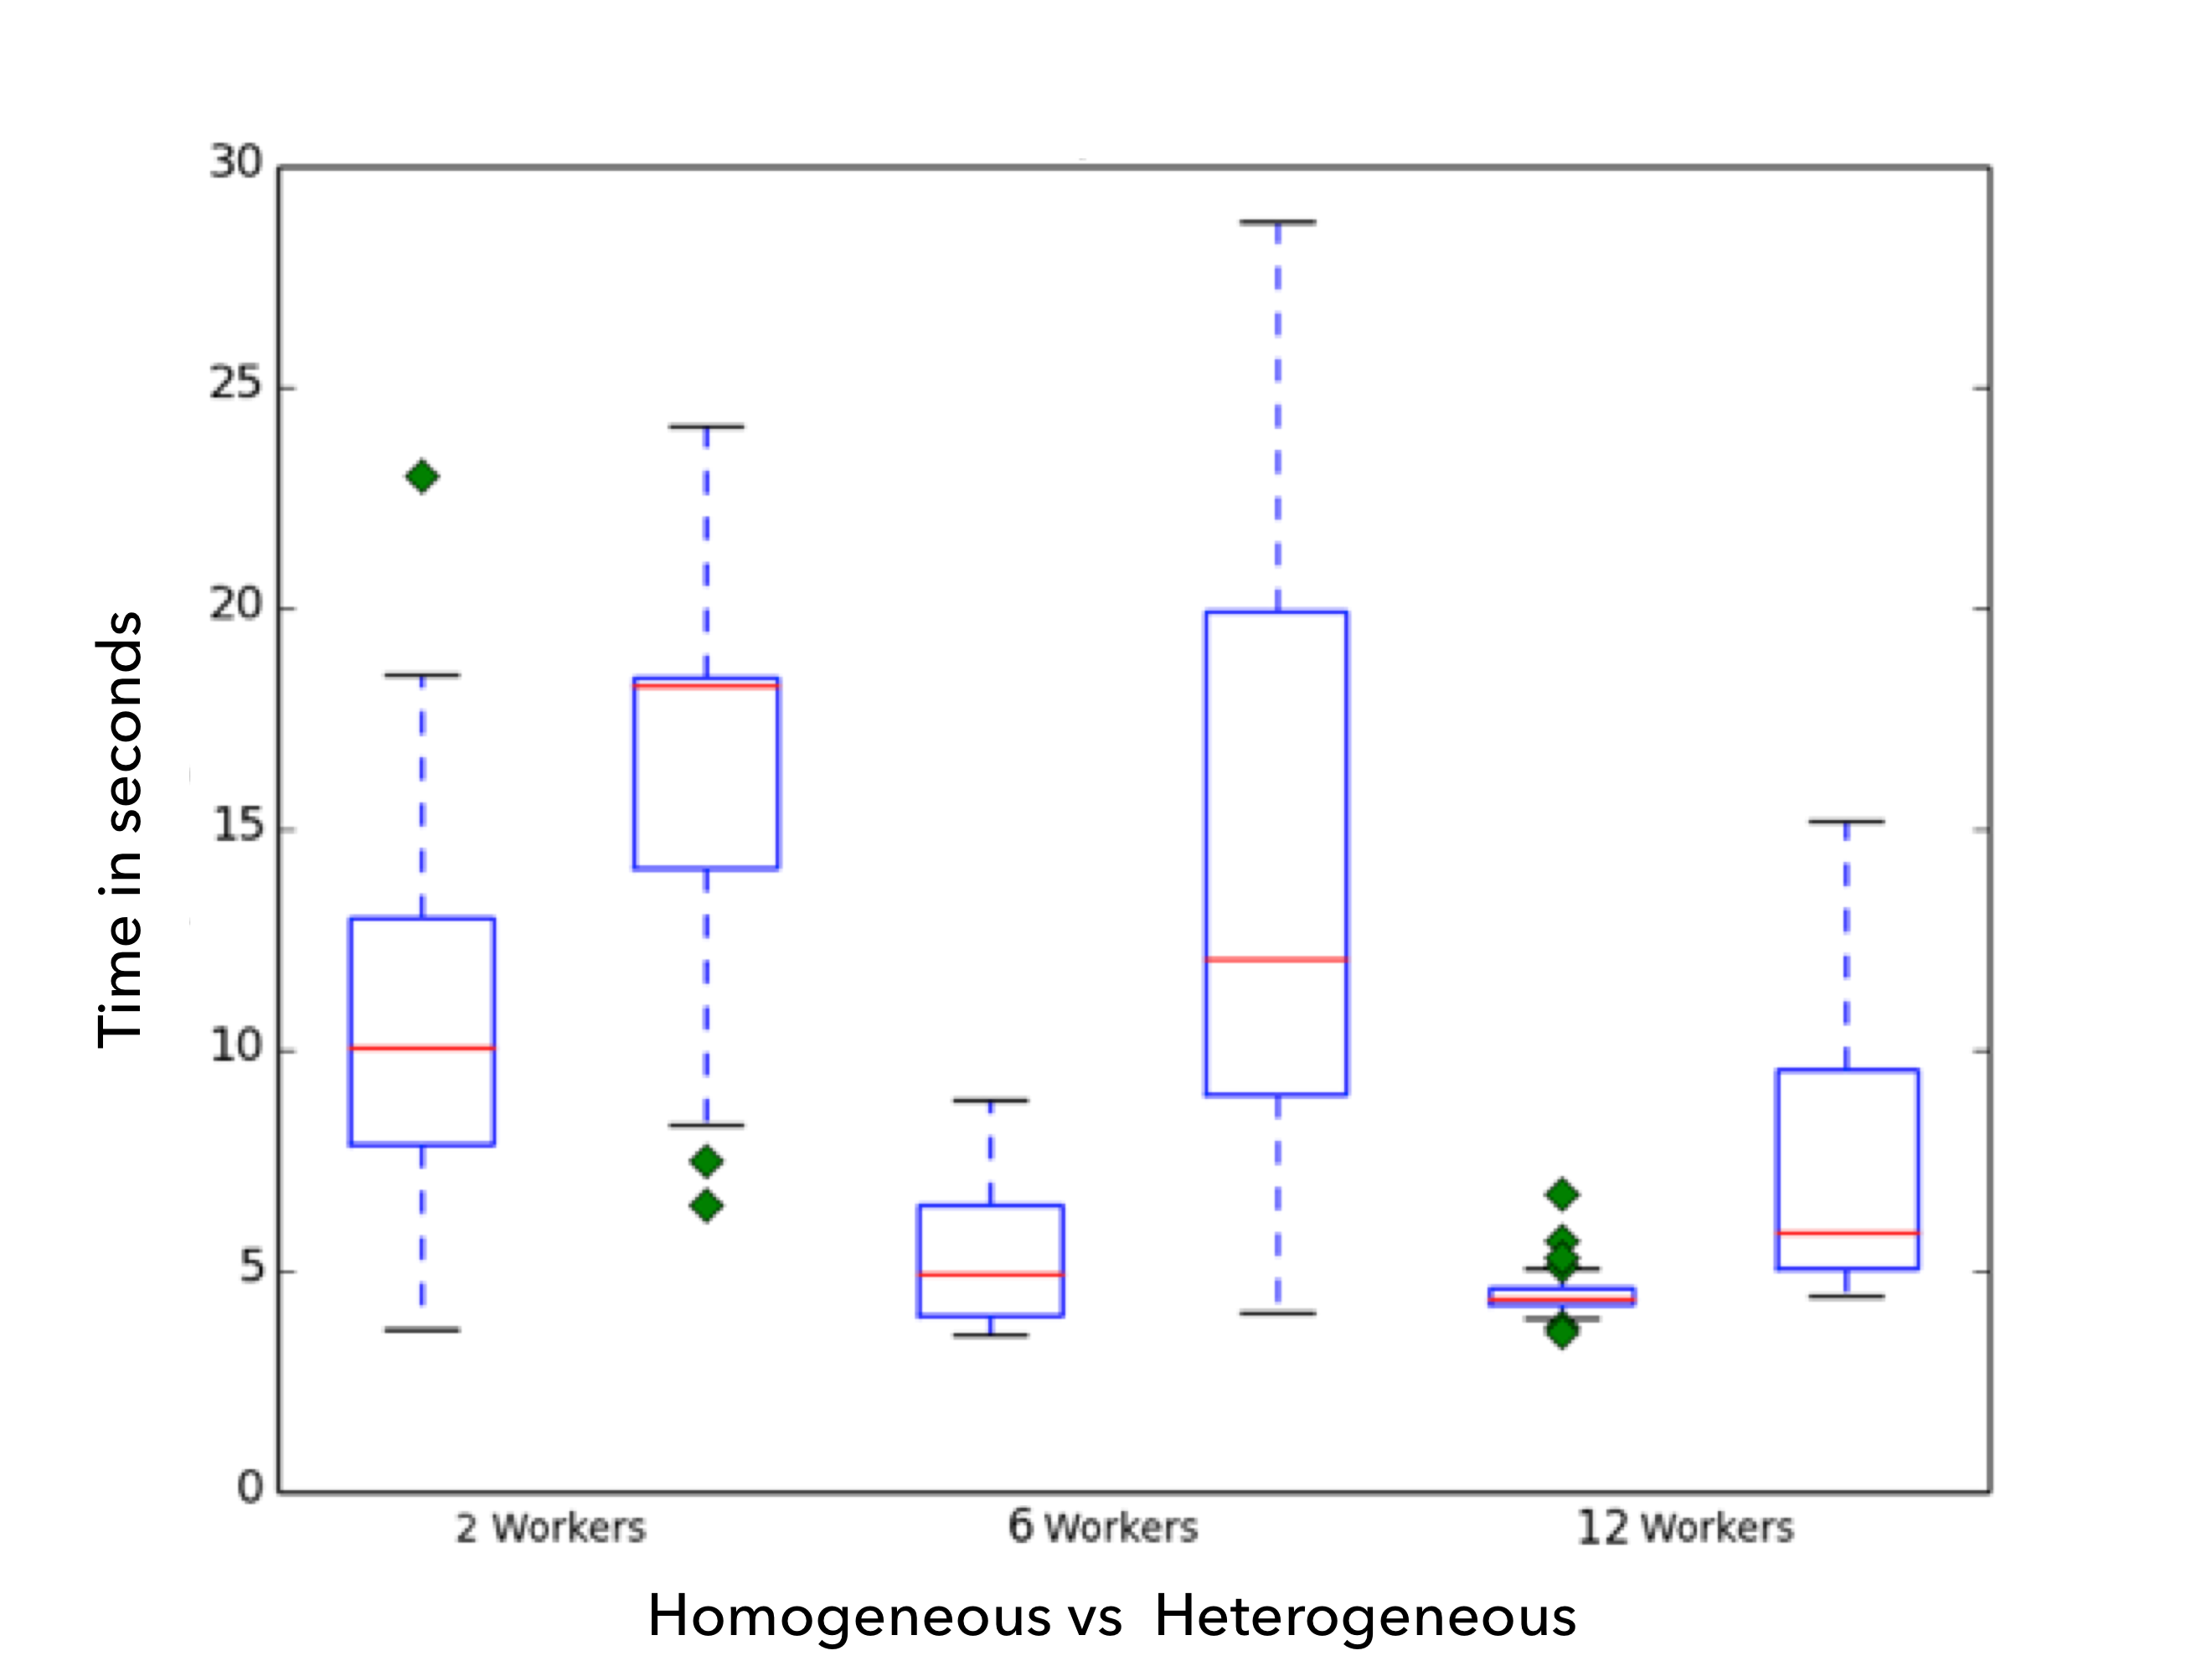
\includegraphics[width=12cm]{img/one_max_comp.png}
    \caption{Comparison of 30 runs of the 128 Bit OneMax problem.
    Box-plot of the number of evaluations needed for solution, with a 2, 6 and 12 workers
    homogeneous configuration as a box-plot to the left of the $x$ axis
    tick, and heterogeneous configuration to the right.
    }
    \label{fig:comp-onemax}
  \end{figure*}
%
\subsection{Results for OneMax}

As mentioned before, the first step is to simulate the manual tuning of the parameters
by running 100 experiments with random parameters and then selecting the best configuration,
using the median performance over 5 runs. Since the OneMax problem is solved by almost all
configurations, performance is determined by the time required to find the optimal solution.
%[FALTA ESPECIFICAR PORQUE SE USO EL TIEMPO AQUI, Y PORQUE EL NUMERO DE EVALUACIONES EN LOS OTROS EXPERIMENTOS]
Figure~\ref{fig:effort} shows the time required for different numbers of EvoWorkers.
It can be observed that even with an homogeneous configuration, as the number of workers
increases solutions are found faster on average, but it is also true
that it the median time needed to find the solution also decreases,
with around 75\% of the experiments finding the solution in the same
amount of time, around 5 seconds, as the bottom chart in the
aforementioned Figure shows.  In general, increasing the number of workers increases
the number of function evaluations carried out over a unit of time. This implies that the selection
of a good configuration could be found easier when using a higher number of workers, relative
to the total wall-clock time.

In Figure~\ref{fig:comp-onemax} the results of 30 runs comparing against the RPSS approach is shown.
It can be observed that as the number of EvoWorkers increases the median of the time decreases, but
in this case the best of the heterogeneous solutions (12 workers) is only better than the worst homogeneous
solution. In this case, the heterogeneous/random configuration
presented in this paper does not obtain better results than the
homogeneous configuration using the best parameters found by random
search. This problem, which is deceptively simple, actually depends
more on the exploitative part than the explorative part. The
heterogeneous worker solution, however, seems to lean more on
exploration by keeping high diversity, something that might not be
actually needed during the last phases of the OneMax problem. This
might be also the case for other combinatorial optimization problem,
but checking the cases when that happens is left as future work.

\subsection{Results for Real-valued Optimization Functions}
%
\begin{figure*}[t]
    \centering
    \subfigure  [6 workers]
    {
        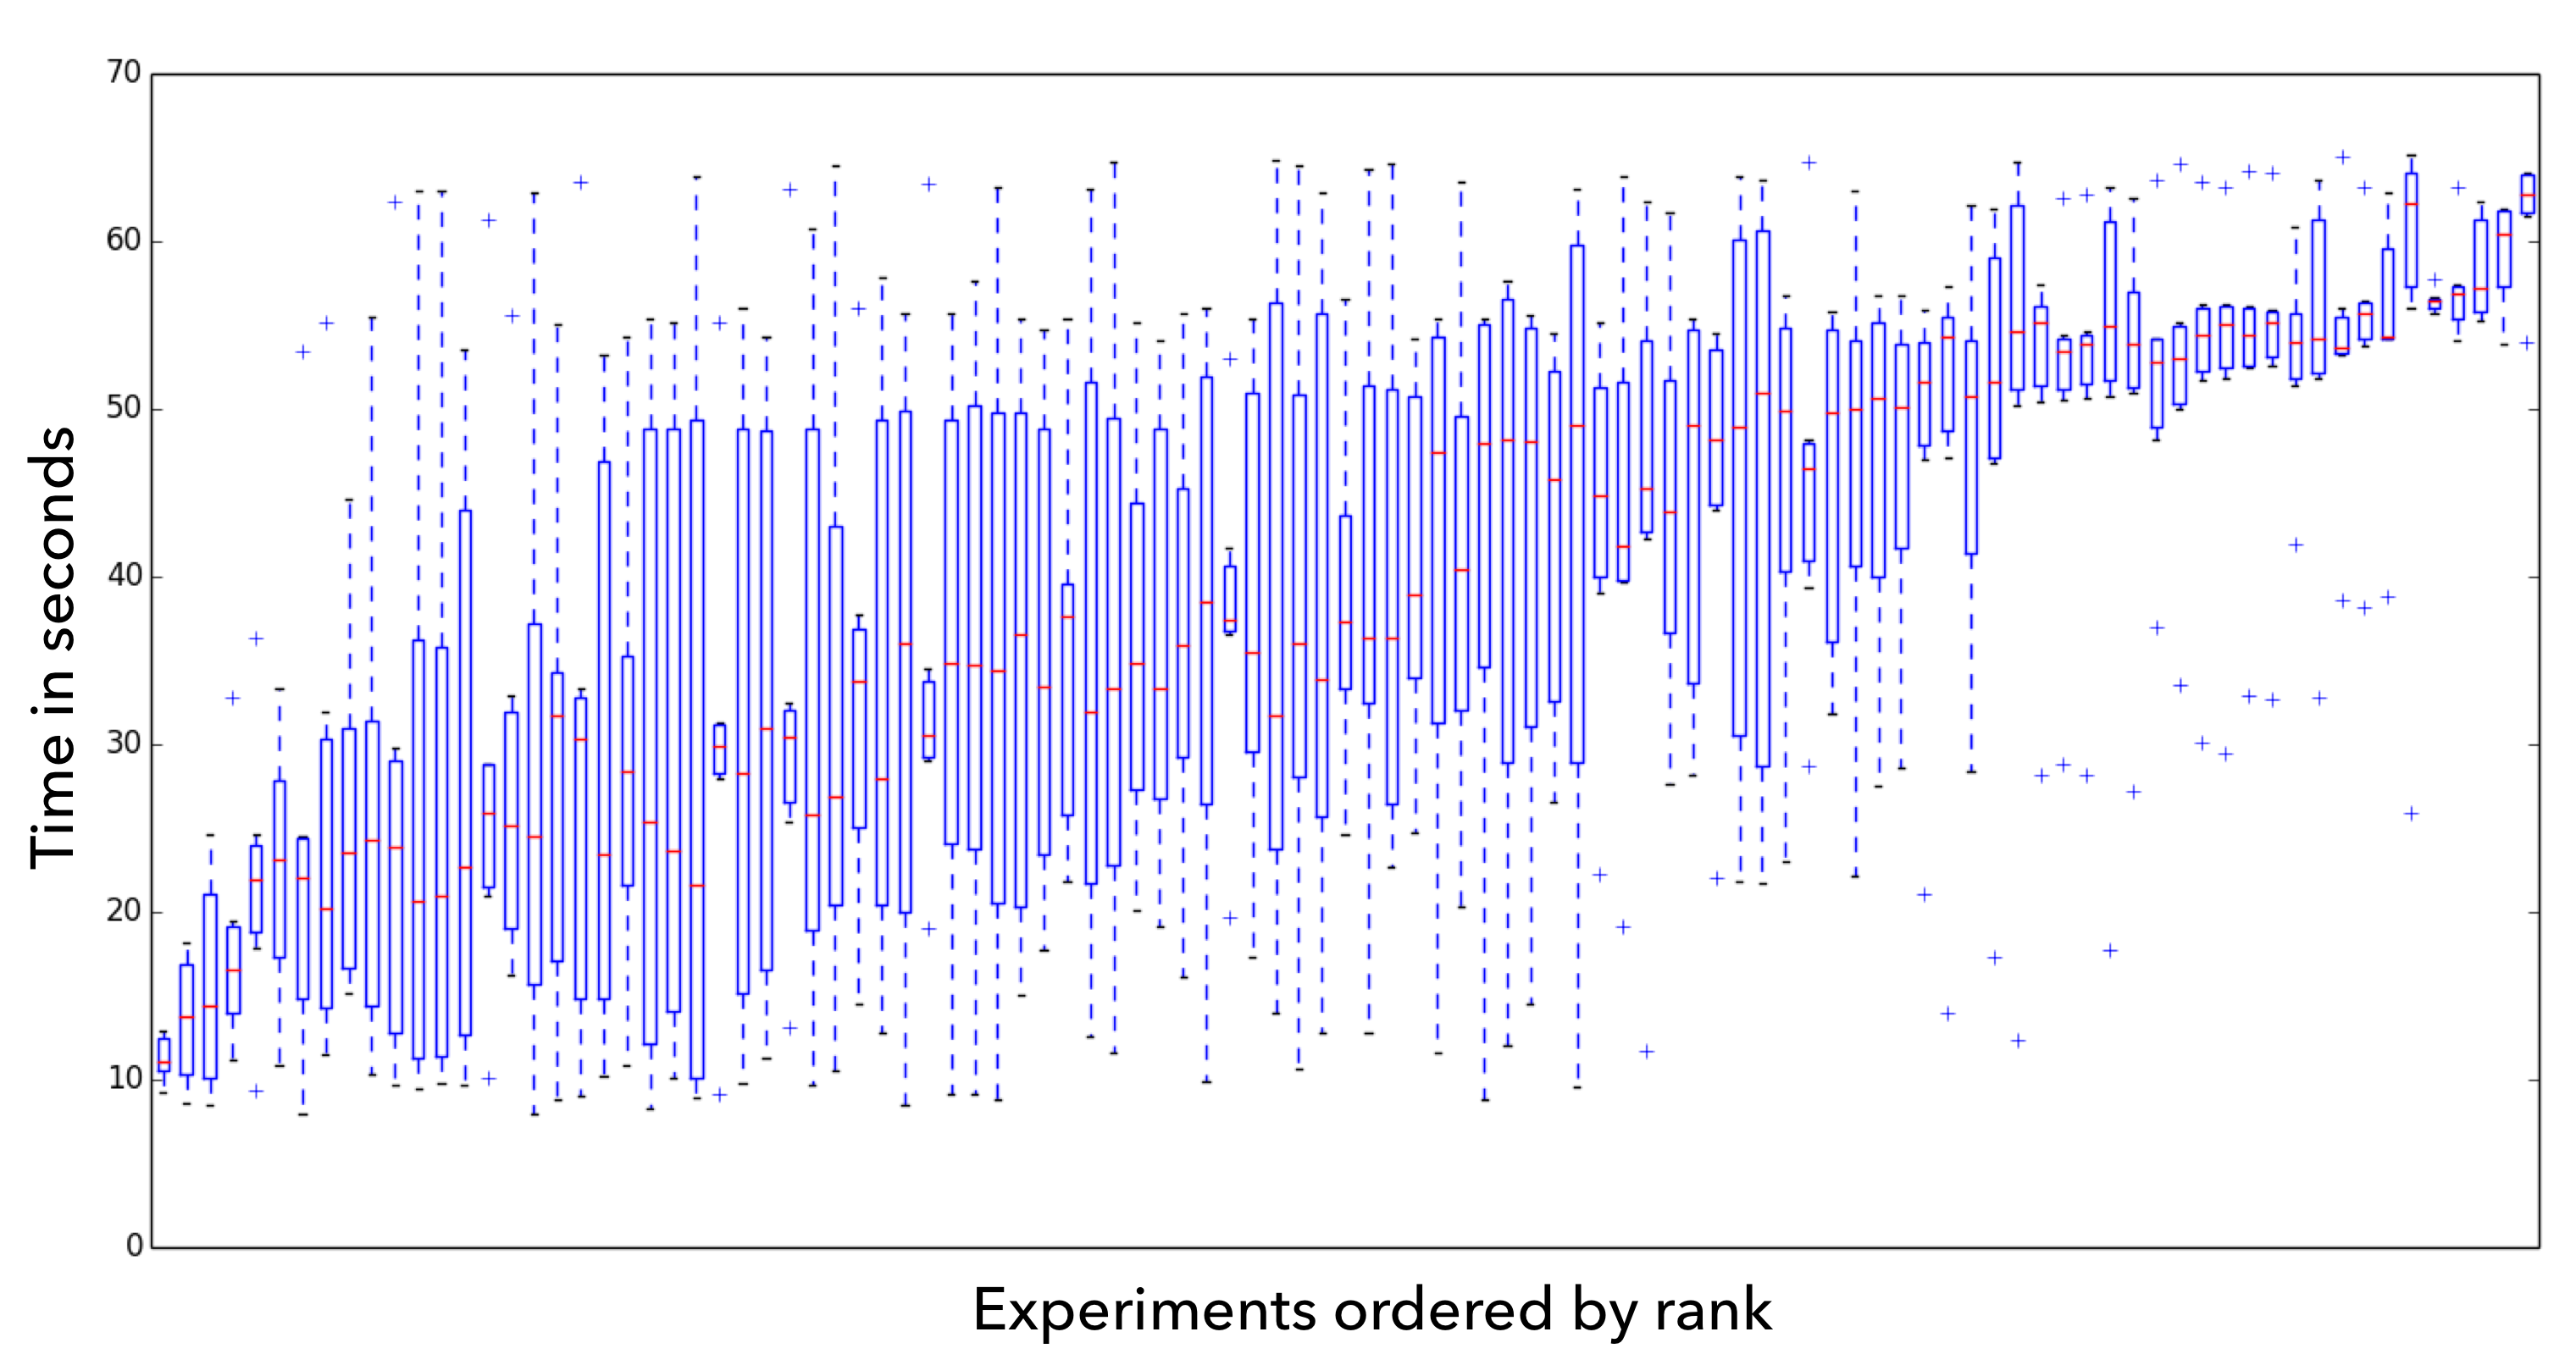
\includegraphics[width=3in]{img/6w_griewank_100_box.png}
    }
    \subfigure  [12 workers]
    {
        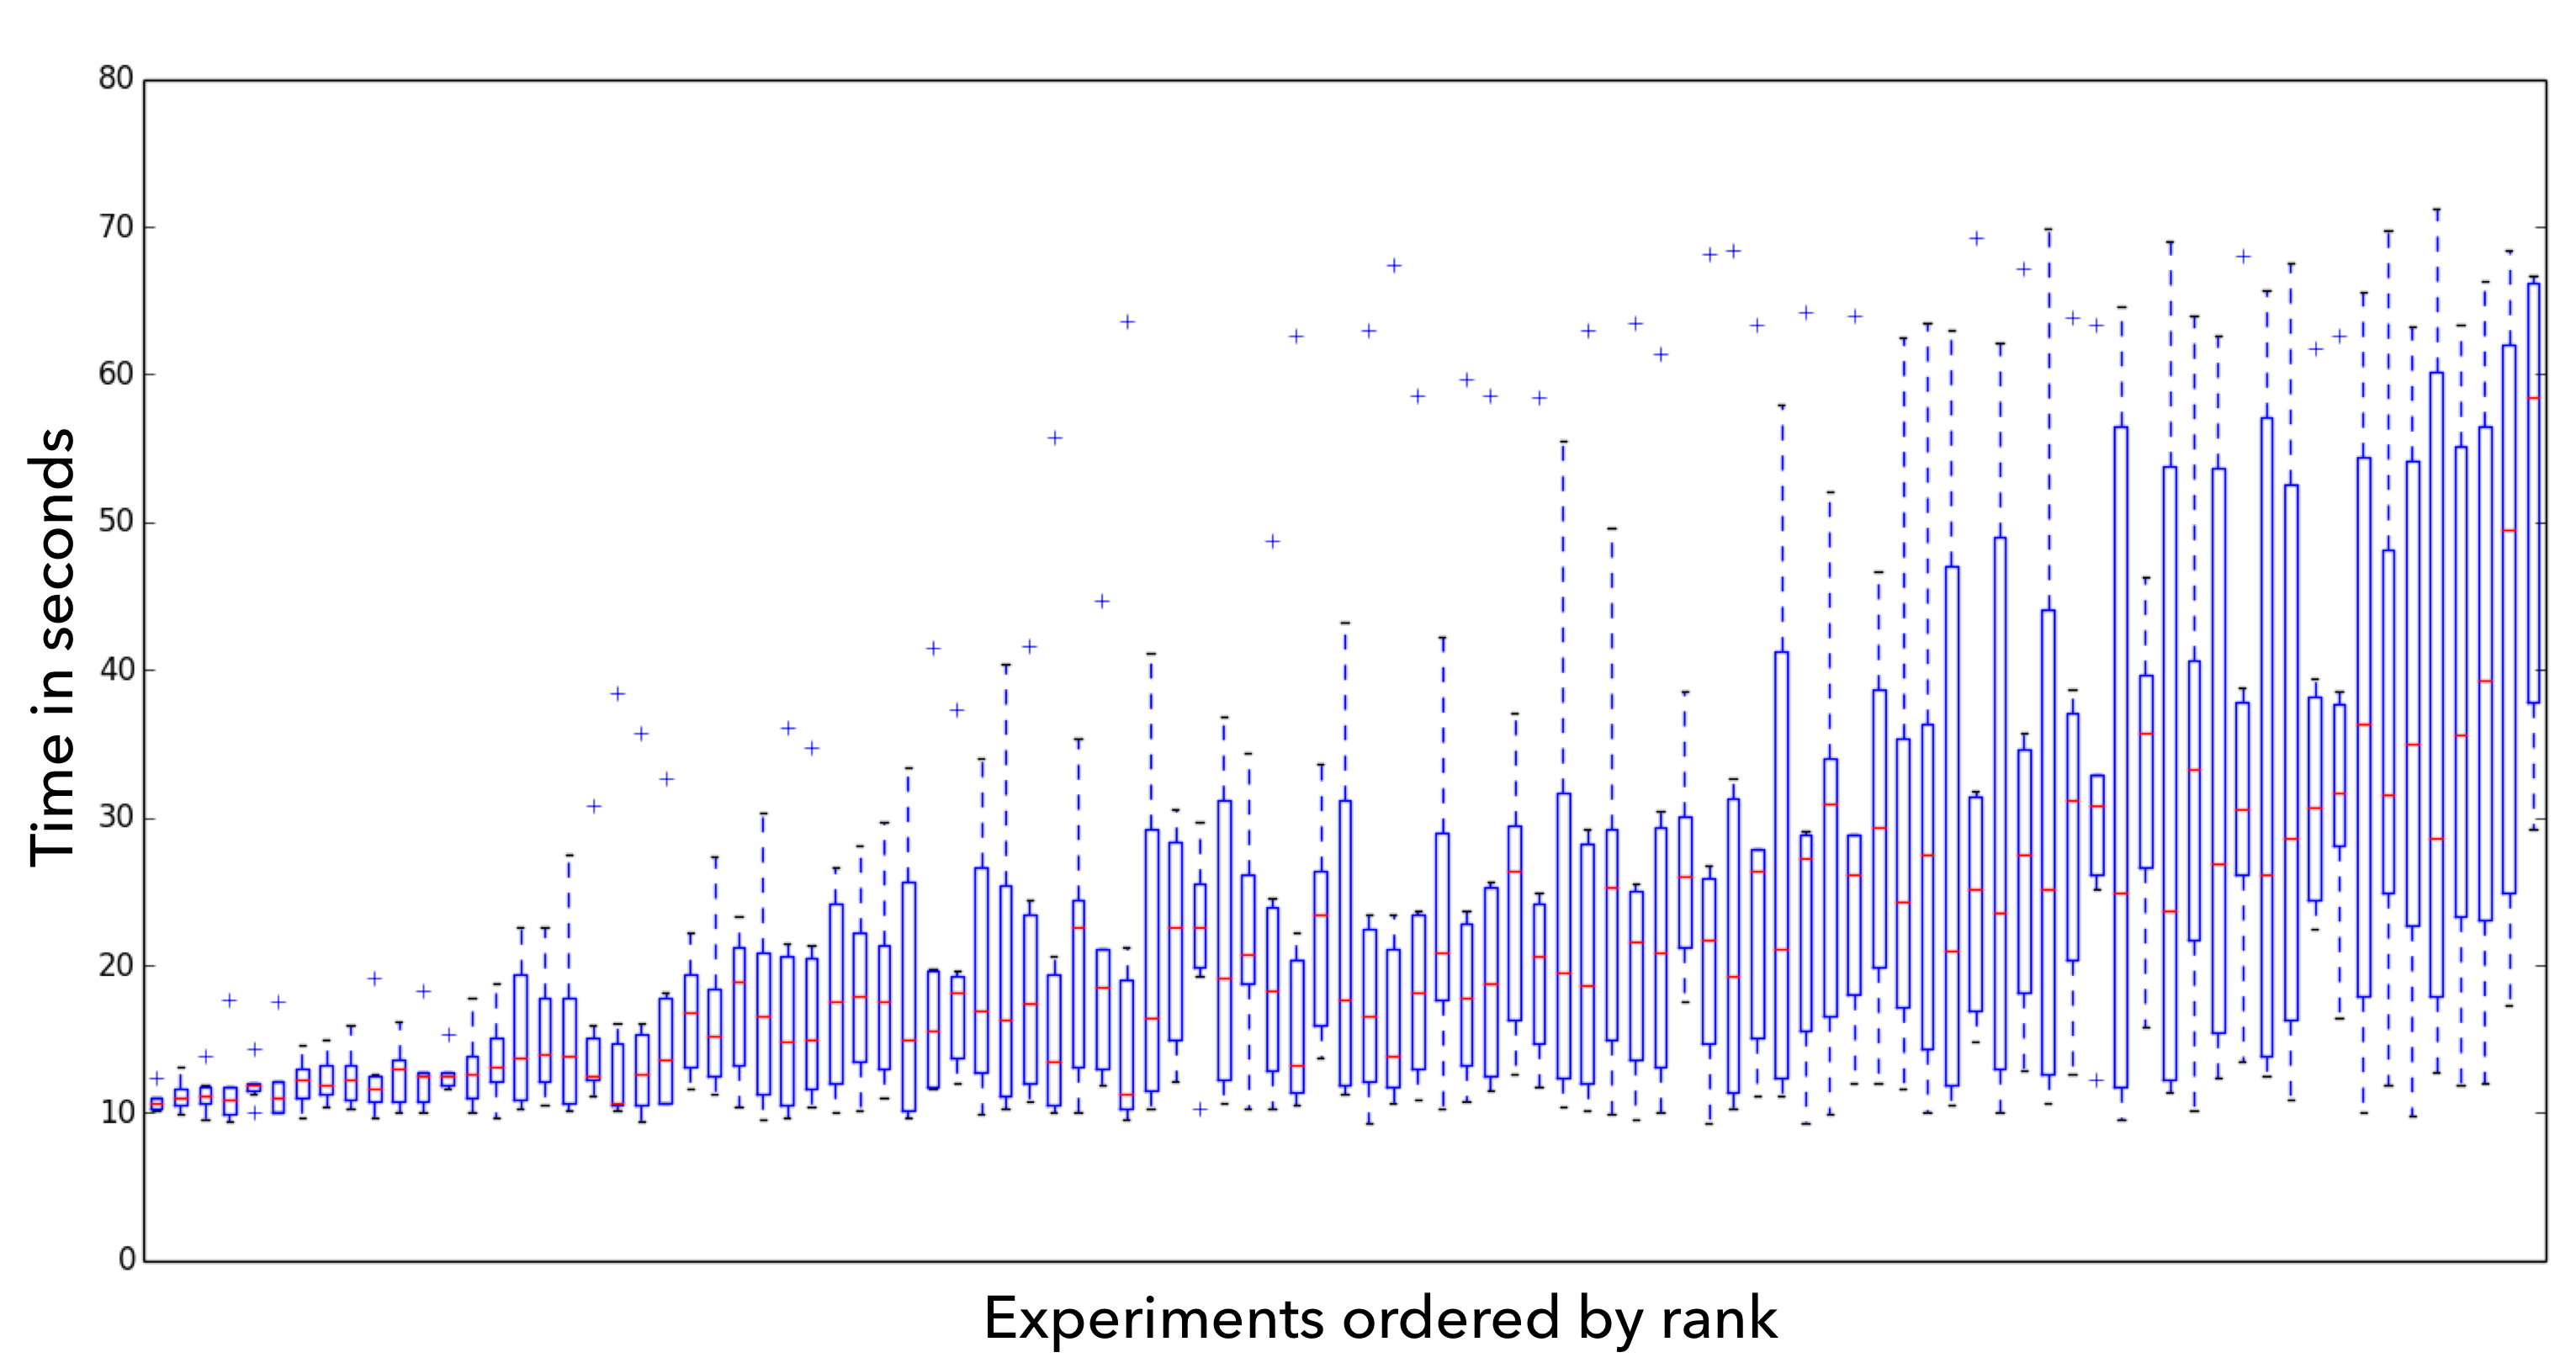
\includegraphics[width=3in]{img/12w_griewank_100_box.png}
    }

    \caption{100 experiments with random parameters for the 100 dimensions Griewank
    real-valued optimization test function. Experiments are ranked by
    the mean time to solution of 5 runs, with (a) 6 workers, and (b) 12 workers.}
    \label{fig:griewank}
\end{figure*}
%
\begin{figure*}[t]
    \centering
    \subfigure  [Homogeneous]
    {
        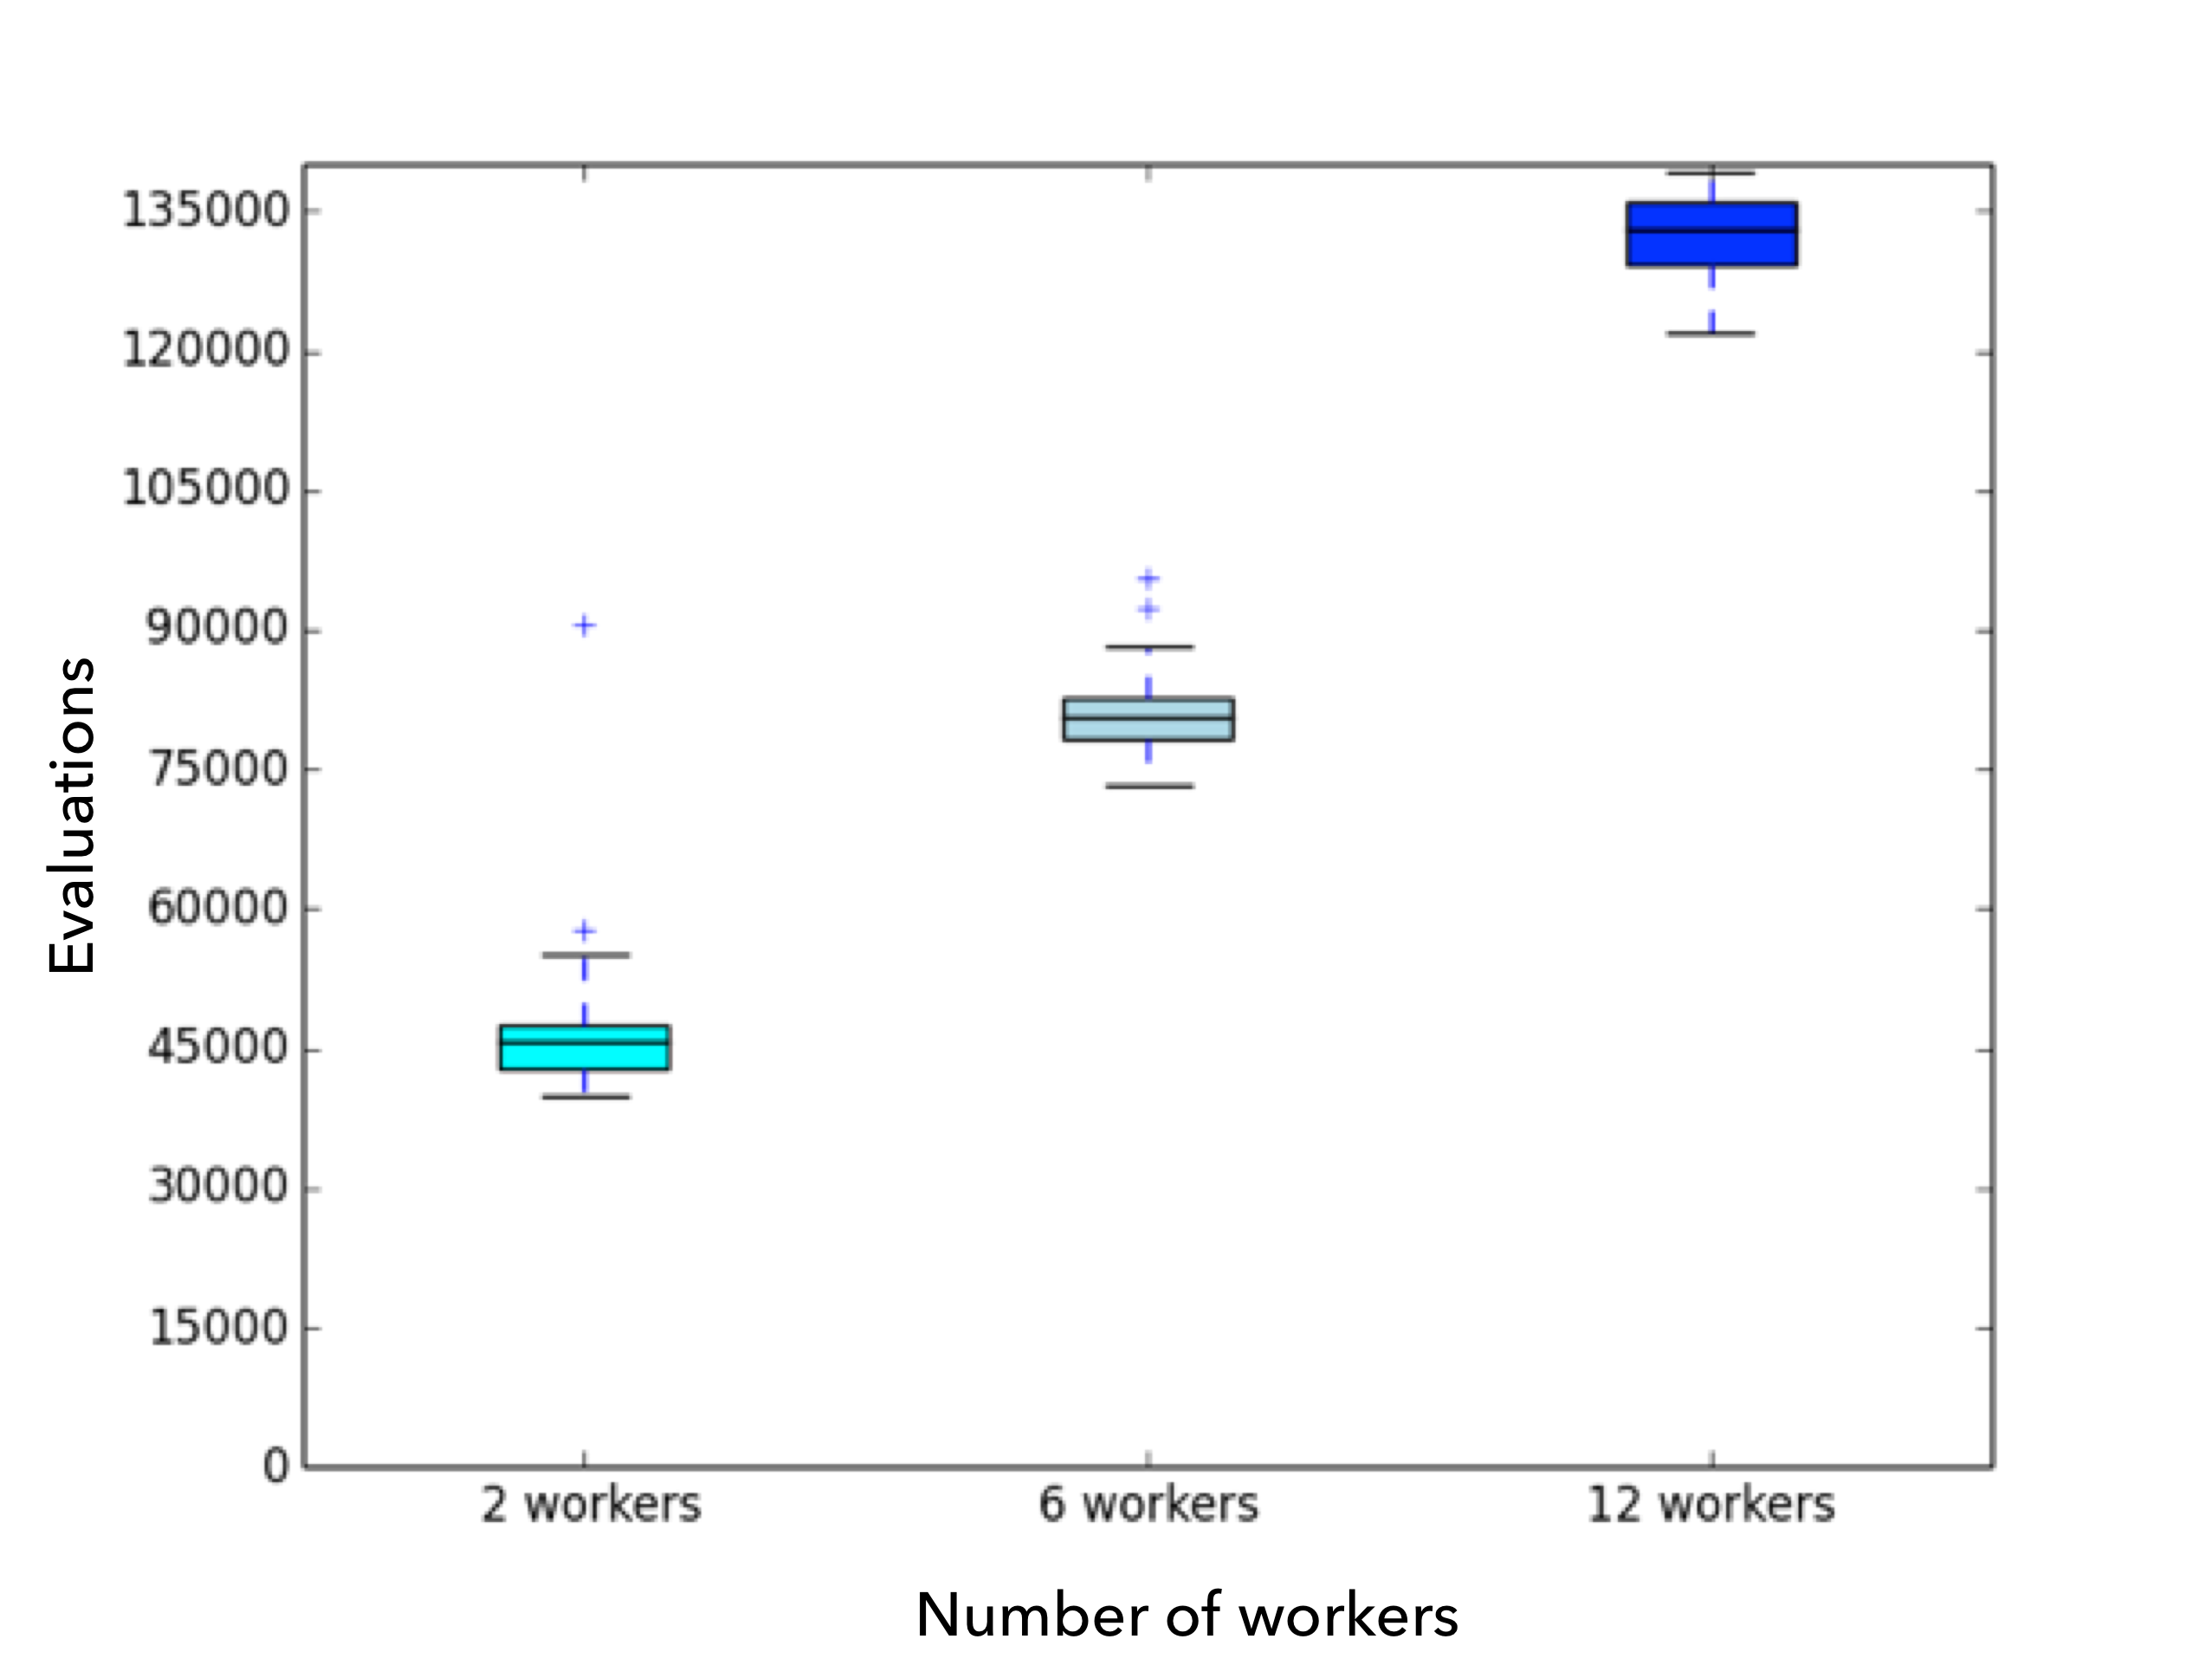
\includegraphics[width=3in]{img/griewank_evals_homo.png}
    }
    \subfigure  [Heterogeneous]
    {
        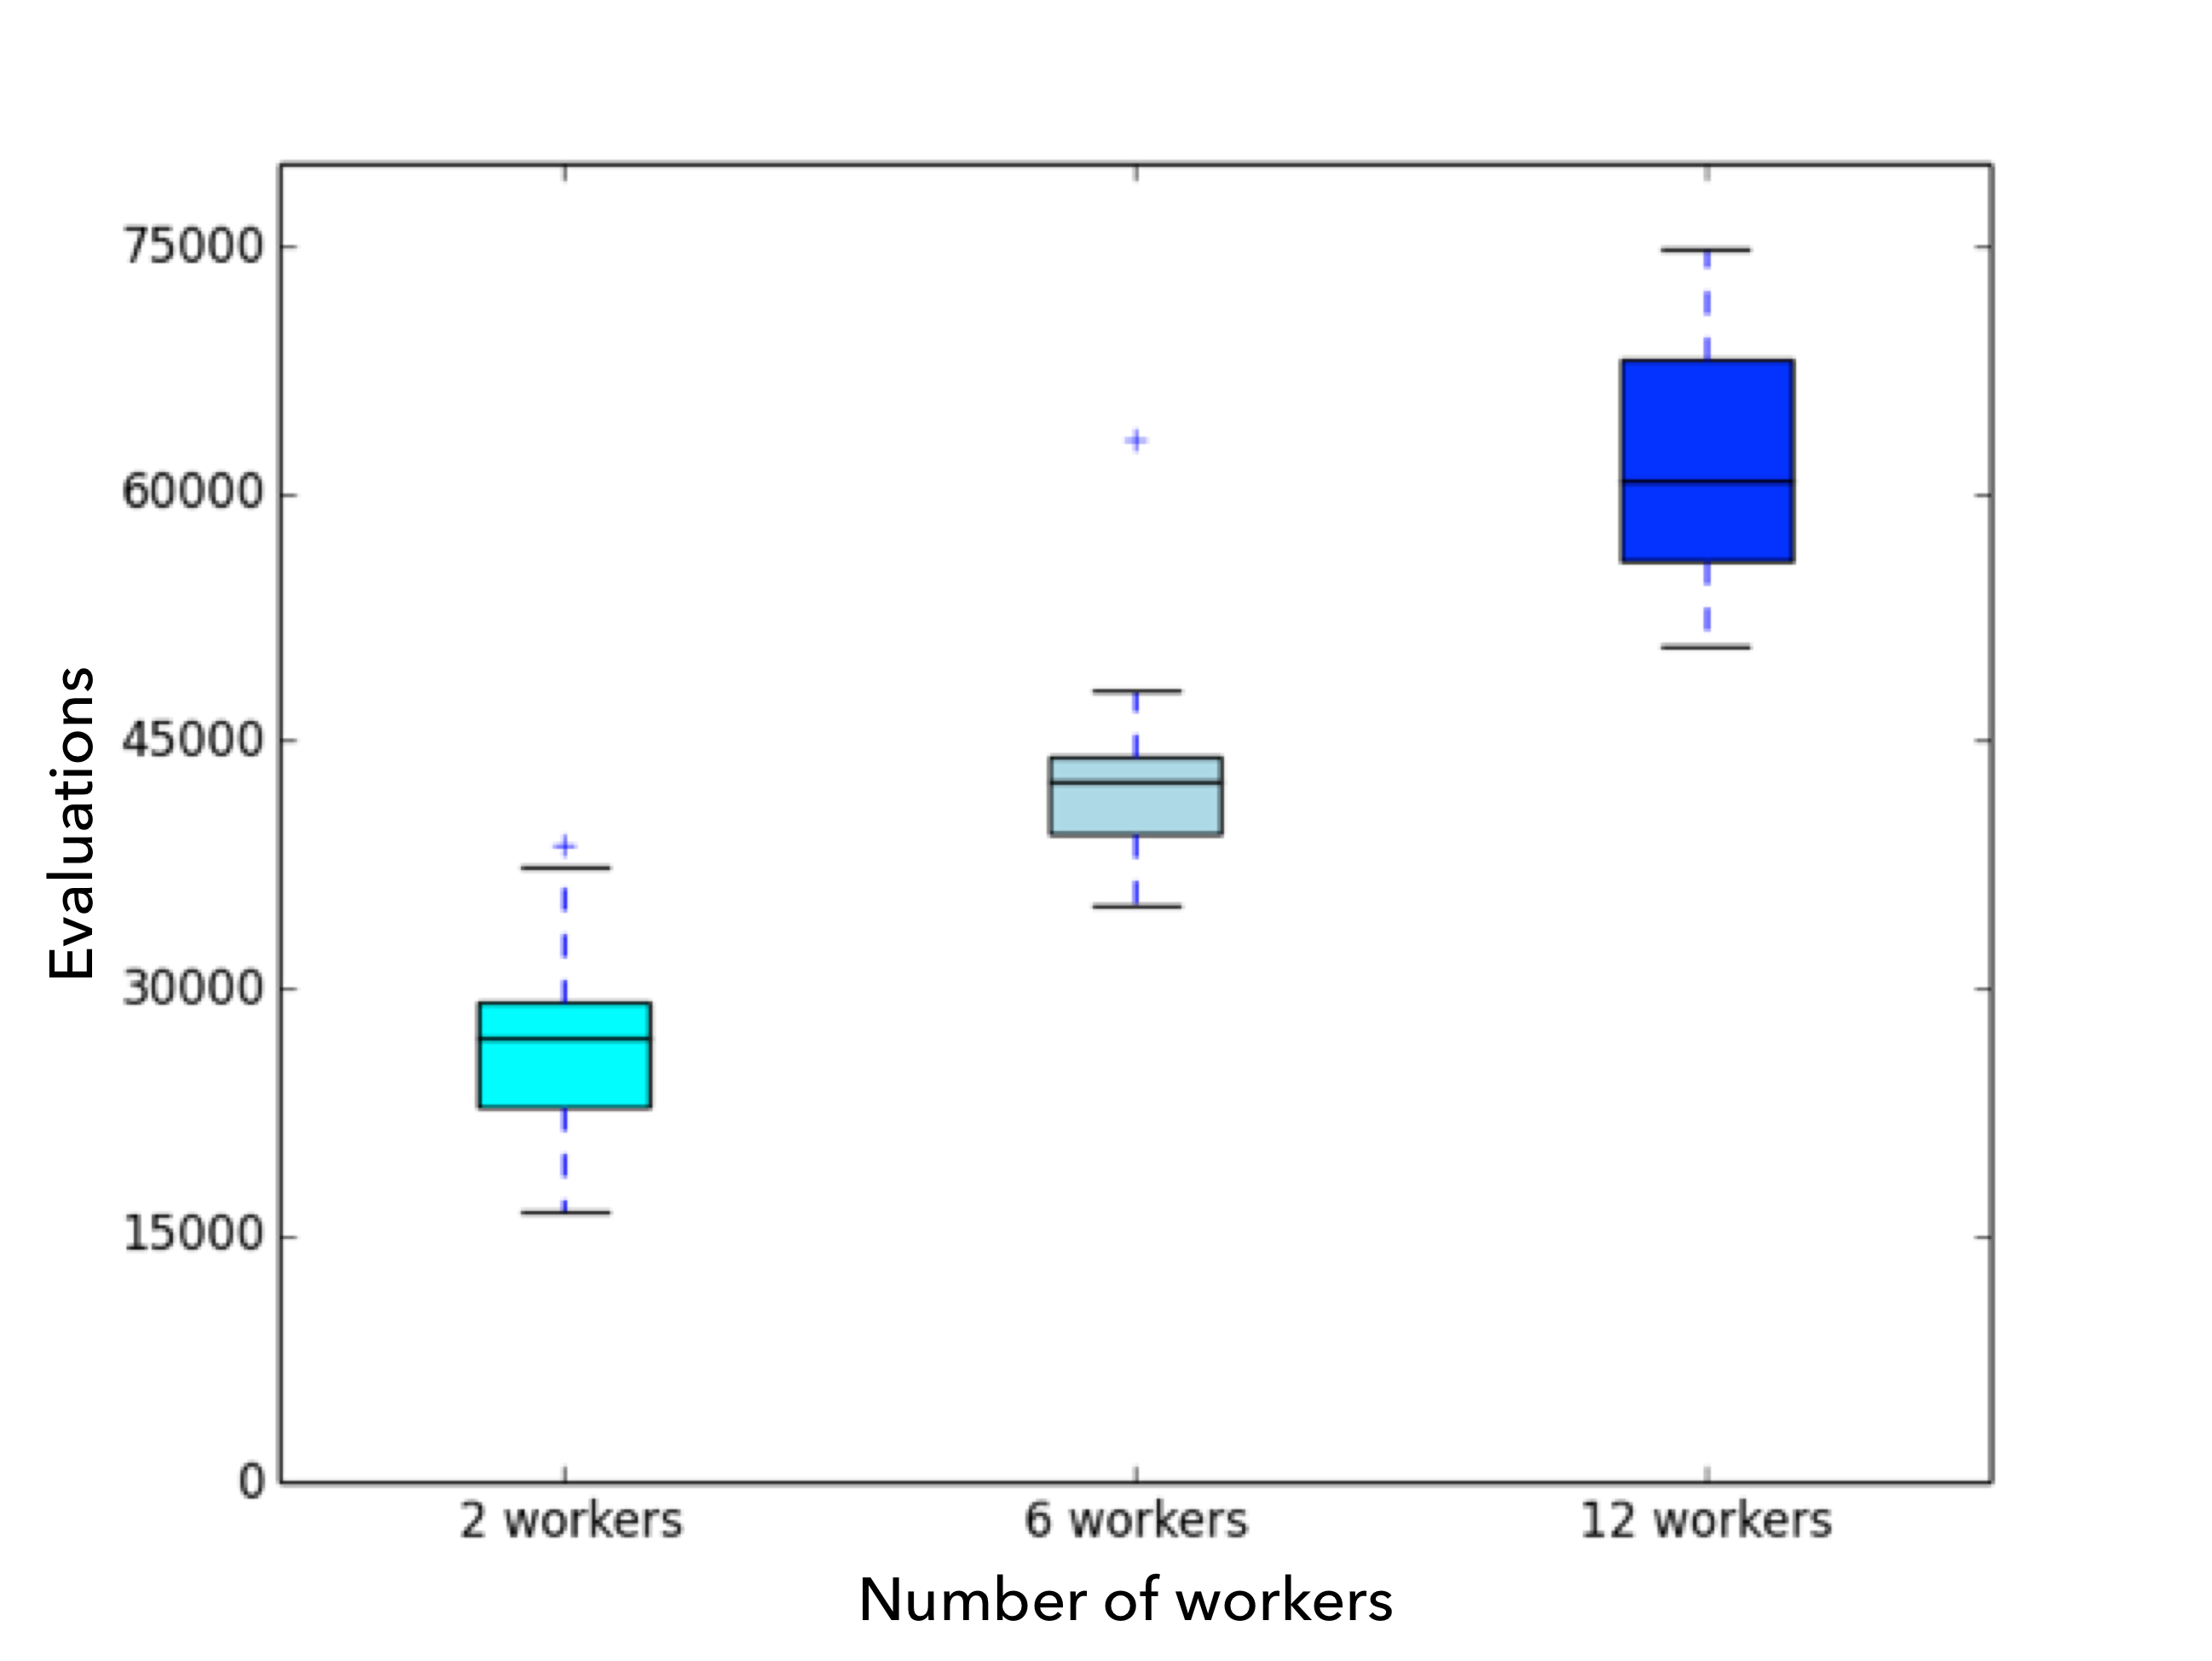
\includegraphics[width=3in]{img/griewank_evals_hetereo.png}
    }
      \caption{ 30 runs on the Griewank function. Box-plot of the number of evaluations needed for solution,
                 with an (a) Homogeneous configuration, and (b) Heterogeneous configuration.}
    \label{fig:griewank-evals}
\end{figure*}
%
\begin{figure*}[t]
    \centering
    \subfigure  [Homogeneous]
    {
        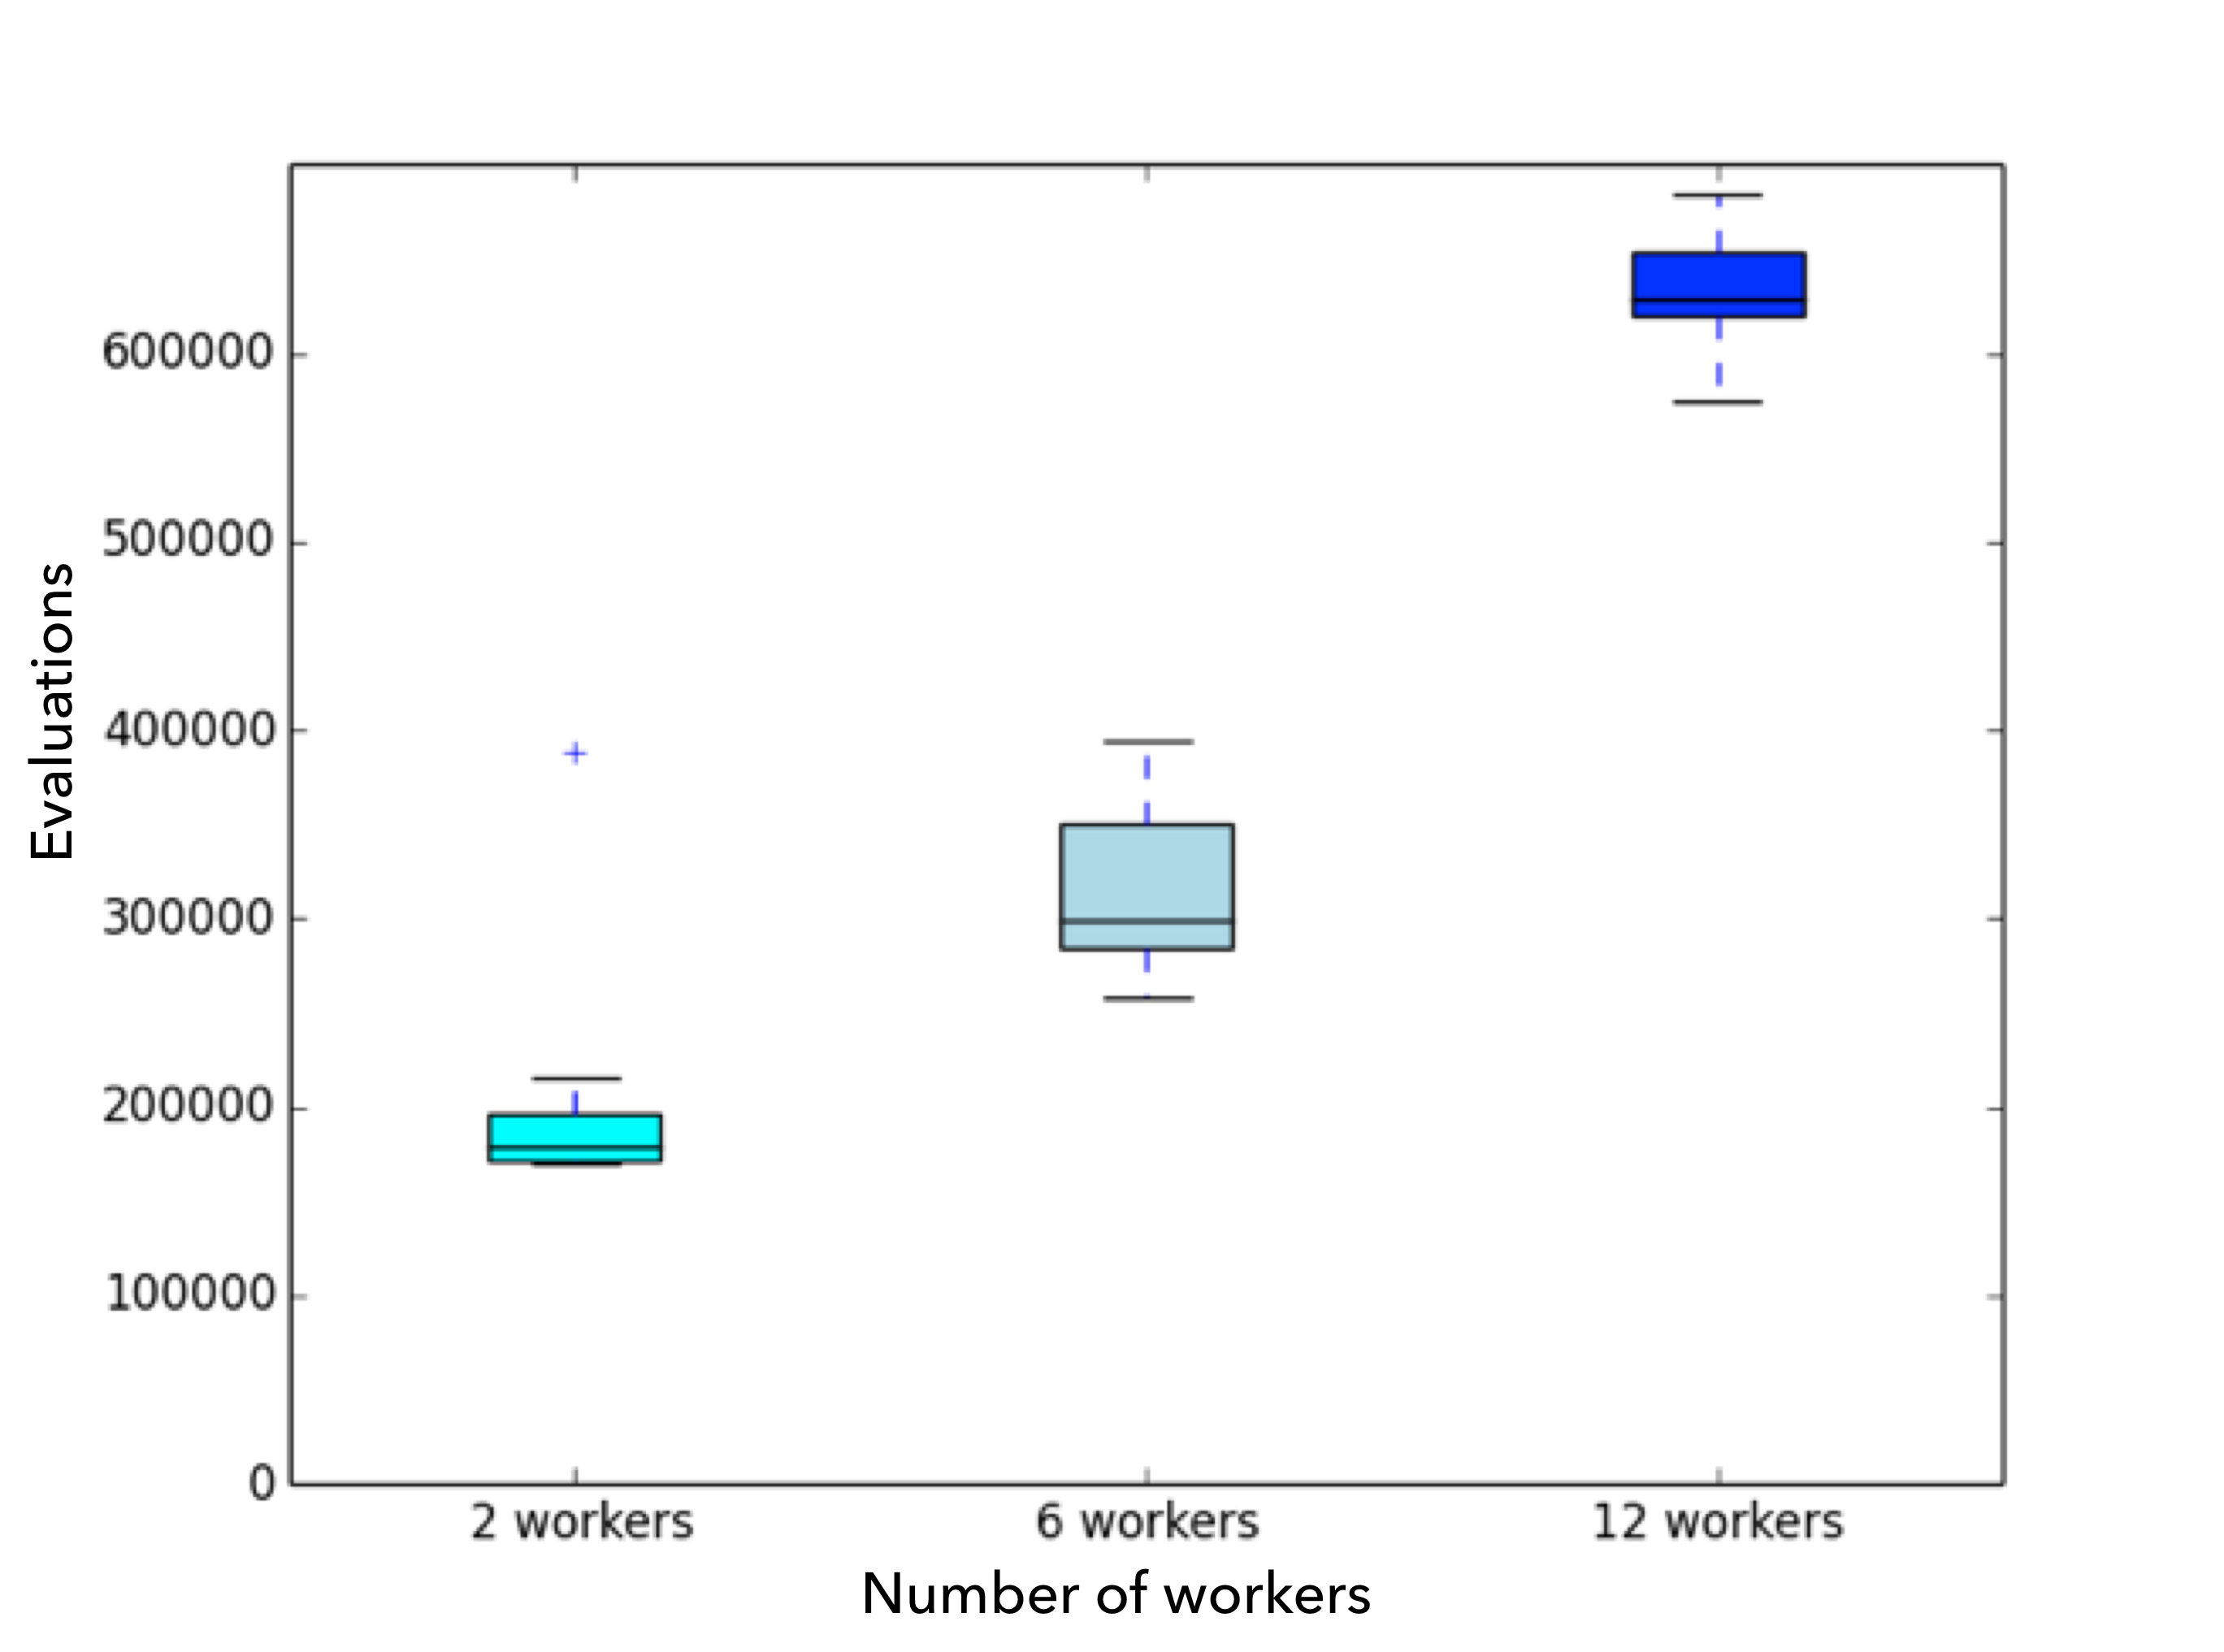
\includegraphics[width=3in]{img/schaffer_evals_homo.png}
    }
    \subfigure  [Heterogeneous]
    {
        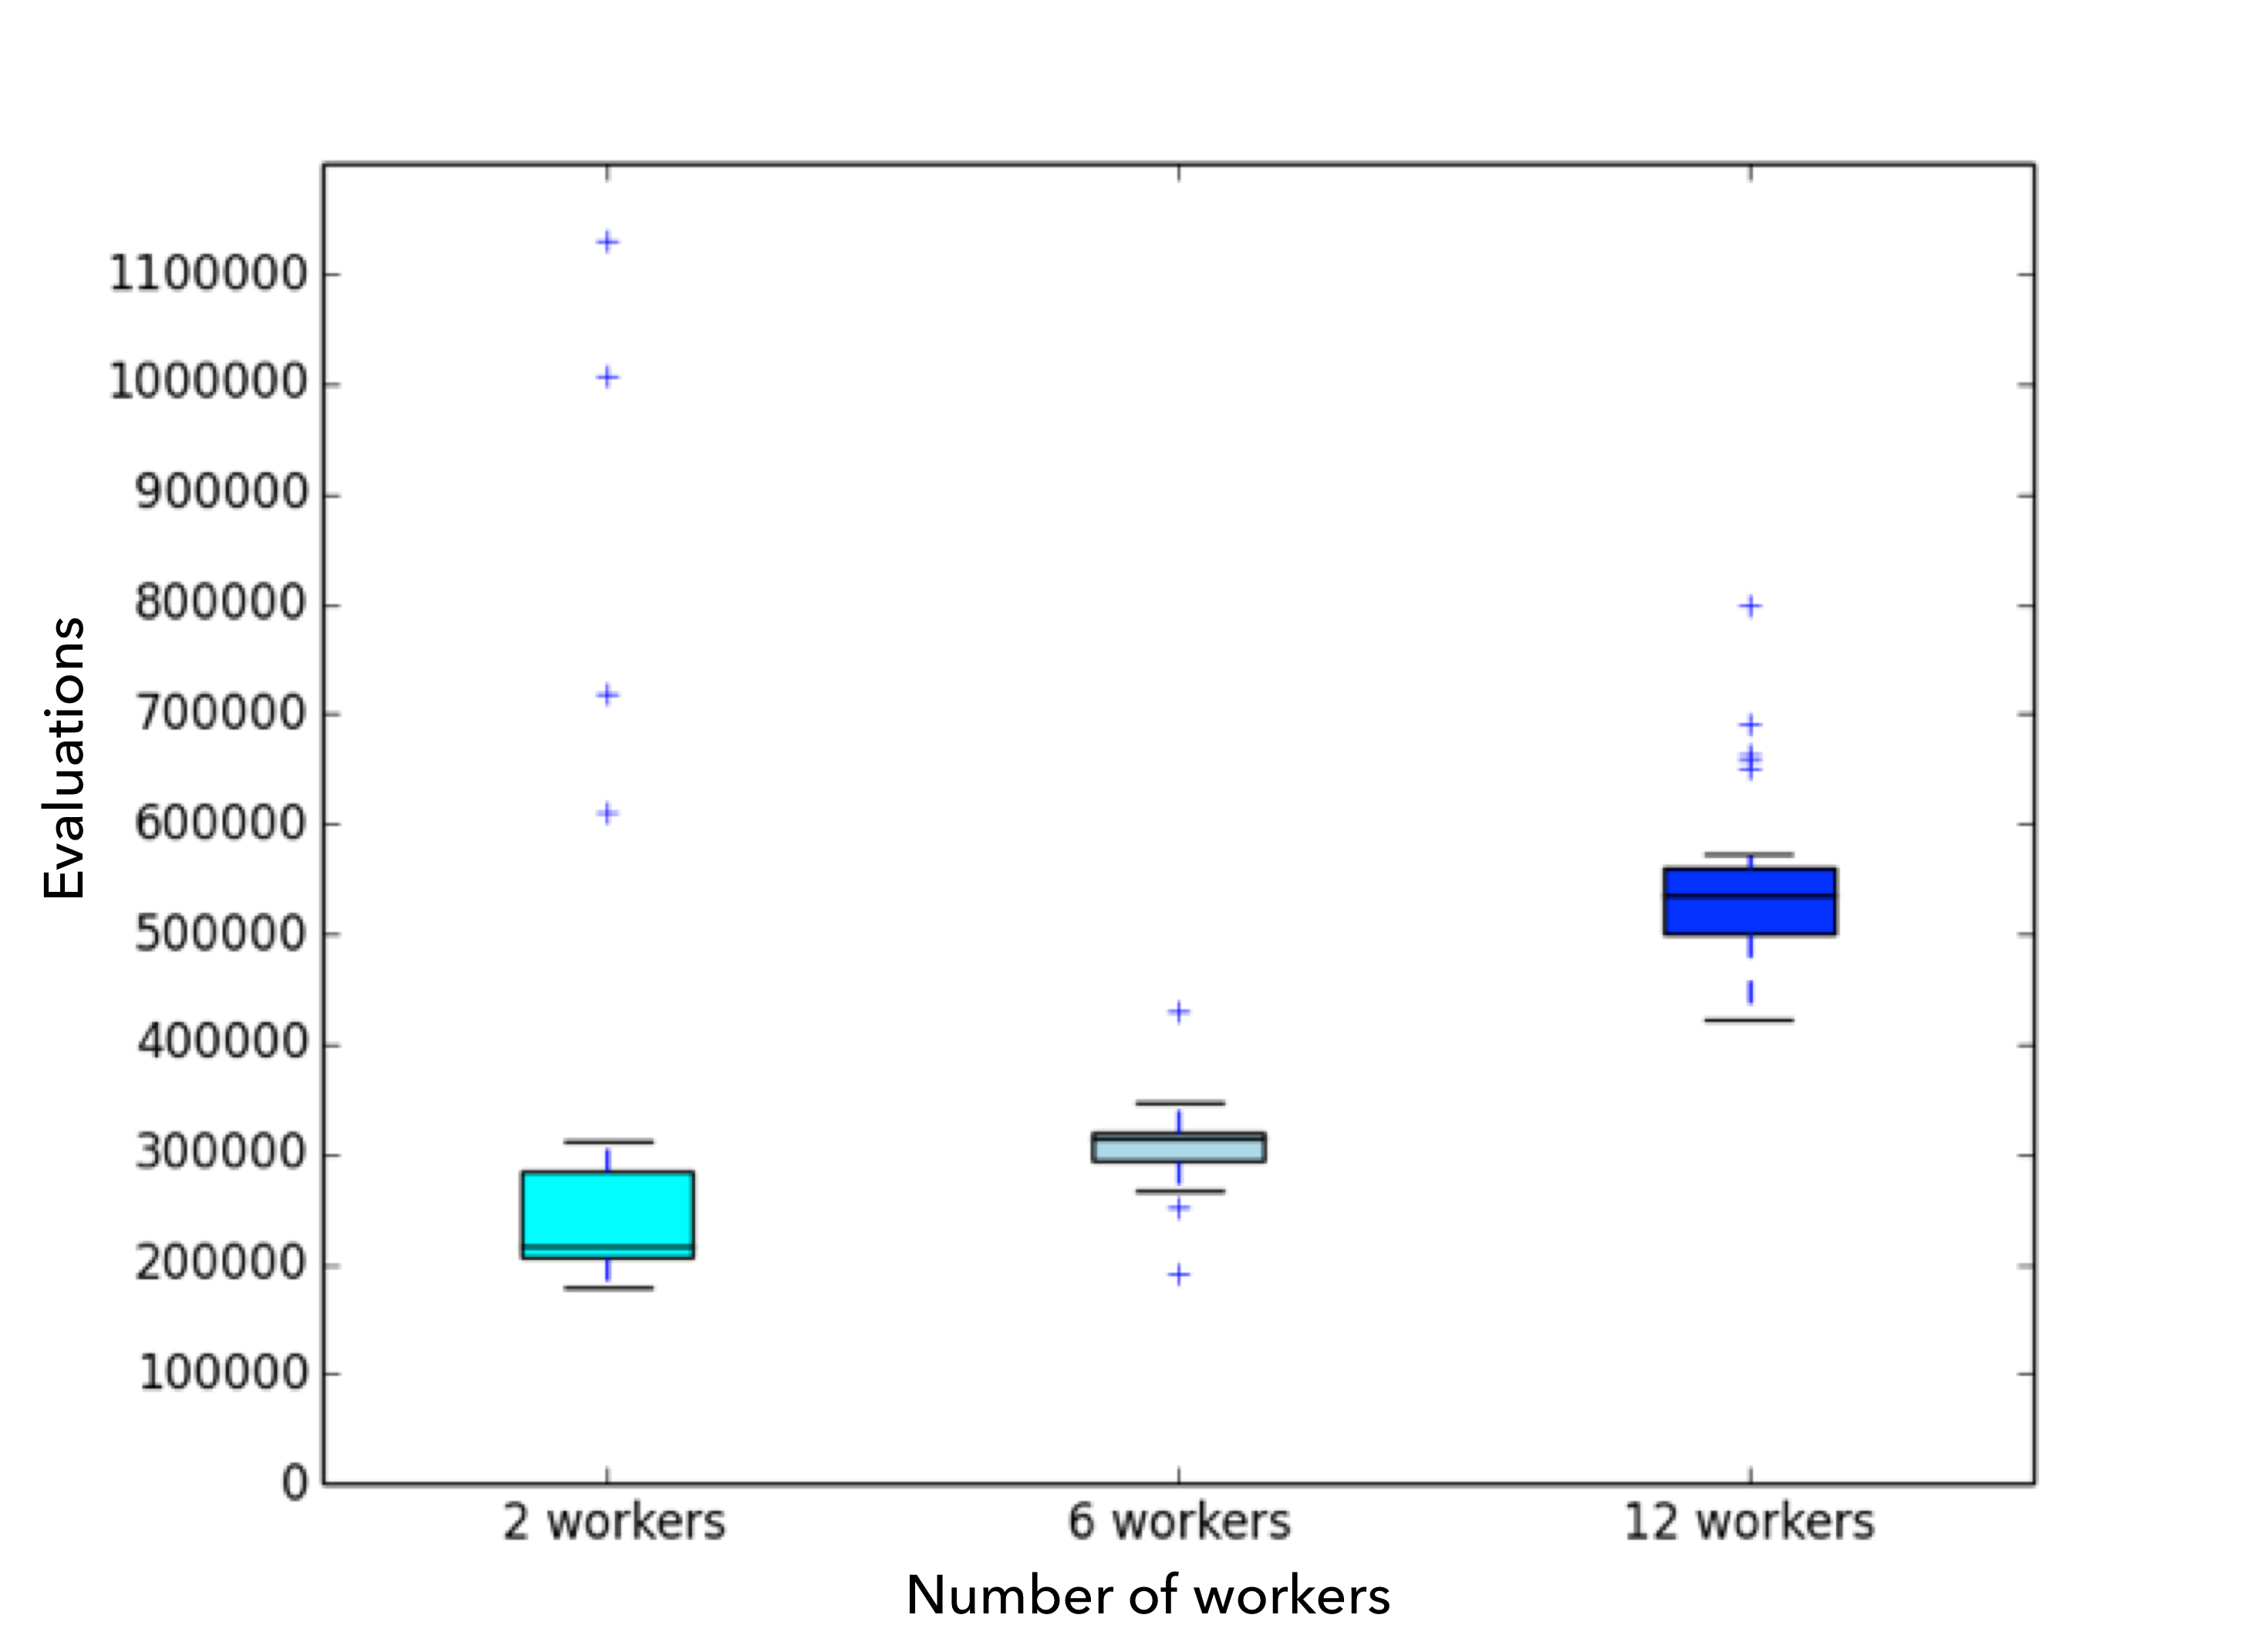
\includegraphics[width=3in]{img/schaffer_evals_hetereo.png}
    }


    \caption{30 runs on the Schaffer function. Box-plot of the number of evaluations needed for
      solution, with an (a) Homogeneous configuration, and (b) Heterogeneous configuration.}
    \label{fig:schaffer}
\end{figure*}
%
\begin{table*}[t]
  \centering
  \caption{Summary of results obtained for the five floating point
      optimization problems. }
    \label{fig:summary}
    \begin{tabular}{|l|l|c|c|c|c|c|c|}
      \hline 
      \multirow{2}{*}{Function} & \multirow{2}{*}{Number of EvoWorkers} &  \multicolumn{3}{|c|}{Heterogeneous} & \multicolumn{3}{|c|}{Homogeneous}\\
      \cline{3-8}
                                & & 2 & 6 & 12 & 2 & 6 & 12\\
            \hline 
      \multirow{2}{*}{Ackley} & Mean time & 8.48& 5.707& 5.290 & 100.595 & 52.171 & 65.2023\\
      \cline{2-8}
                                & Mean evaluations & 27534.30 & 40239.66 & 60466.16 & 47645.9 & 81388.9 & 132308.6 \\
      \hline 
      \multirow{2}{*}{Rastrigin} & Mean time &  128.486207 & 36.847931 & 14.43517241 & 8.46793103 & 11.8510345 &  4.43517241 \\
      \cline{2-8} 
                                & Mean evaluations & 457148.552 & 347344.379 & 218830.552 & 31697.6897 & 105434.966 & 56090.7931 \\
      \hline
      \multirow{2}{*}{De Jong} & Mean time & 37.2465517 & 17.382069 & 17.6596552 & 33.1886207 & 19.77 & 27.2806897 \\
      \cline{2-8}

                                & Mean evaluations & 156795.276 & 213783.345 & 330531.828 & 159259.655 & 281918.034 & 651978.345 \\
      \hline
      \multirow{2}{*}{Griewank} & Mean time & 8.27241379 & 5.5337931 & 5.30482759 & 7.645667 & 5.716667 & 5.617333 \\
      \cline{2-8}

                                & Mean evaluations & 23688.8966 & 37118.1034 & 59249.2759 & 25779.6 & 42953.33 & 70536.53 \\
            \hline

      \multirow{2}{*}{Schaffer} & Mean time &  89.6493103 & 37.3044828 & 29.8093103 & 55.2410345 & 34.4448276 & 36.7113793 \\
            \cline{2-8}
                                & Mean evaluations & 316702.552  & 338147.103 & 545480.793 & 191024.759 & 311083.276 & 637198.31 \\
            \hline

       \end{tabular}

\end{table*}

The same steps as the previous section were followed when evaluating the five real valued
optimization problems of this section.  For brevity only two representative functions are
presented with figures, and summary of all the results are shown in Figure~\ref{fig:summary}. As before
the first step is to tune the parameters for the homogeneous configuration.
In Figure \ref{fig:griewank}, the results of the tuning phase for 6 and 12 workers
for the Griewank function are shown. For 12 workers results are not as flat as before,
with times comparable to the 6 worker configuration in the best case.

To compare the performance of the homogeneous approach and the heterogeneous approach based on RPSS,
Figure \ref{fig:griewank-evals} compares the approaches based on the total number of function
evaluations required to find the optimal solution (with a ).
%[SE DETIENE CUANDO SE ENCUENTRA EL OPTIMO, O CUANDO ESTAS CERCAS POR UN epsilon ?]
% Optimo con hasta 7 decimas - Mario
These results show a clear performance improvement, with the heterogeneous configuration
reducing the total number of function evaluations required to find a solution,
independently of the number of workers used.
On the other hand, for the Schaffer function, performance is quite similar,
with the heterogeneous approach only providing a slight reduction in the number
of function evaluations for the case with 12 EvoWorkers.
In the summary shown in Table ~\ref{fig:summary} two extreme cases are found, the Ackley and Rastrigin functions.
In the former, the heterogeneous configuration achieves the best performance, while the opposite is true on the latter.
Finally, performance on the De Jong function also favors the heterogeneous configurations.

% Maybe try to explain that? - JJ
\section{Conclusions and Further Work}
\label{sec:conclusions}
This paper presents an evaluation of the RPSS parametrization approach on
a pool-based EA, using the OneMax problem and five real-valued optimization functions
in high dimensional space.
Using the RPSS approach, it seems that a PEA can be executed successfully
without any form of parameter tuning, achieving comparable results to standard homogeneous
parametrizations that were tuned for each problem.
Results also show that the benefits of a RPSS are not only present
when using an heterogeneous approach, even a random homogeneous configuration could bring
benefits. Unfortunately the RPSS strategy is not a silver bullet, as there are cases
when it is not the best approach. However these disadvantages are
offset by the fact that it comes very close to zero parameter tuning,
giving a consistently good result across a good range of problem instances.
The worst result is achieved for the Rastrigin function, which
is one of the most difficult ones; not only the time needed is worse,
also the number of evaluations. In case such as these it would be
interesting to use some technique to constrain the range of variation
of the random parameters.

The work presented in this paper, thus, extends the work by Fukunaga
and coworkers by confirming his result in a pool-based environment and
different kinds of fitness functions. In general, we can conclude that
random parametrization will allow a good initial result for most
problems, providing a fast solution in cases where there is not enough
time to perform optimization of the parameters in a parallel setup.

% Future lines of work will focus on using other EA or meta-heuristic techniques,
% such as genetic programming or particle swarm optimization for having
% workers that are heterogeneous in more than one sense. RPSS could be
% used in those cases where each algorithm has different sets of
% parameters, but also to randomly select the technique used in each
% node. Another interesting line of work is the dynamic adaptation of
% parameters by measuring the diversity of each worker or returned
% sample. This could be specially useful in cases where the random
% parametrization technique seems to achieve bad results.

\section*{Acknowledgements}

This paper has been supported in part by project DeepBio (TIN2017-85727-C4-2-P).
% This should be updated


%----------------------------------------------------------------------------------------
%	REFERENCE LIST
%----------------------------------------------------------------------------------------
\bibliographystyle{IEEEtran}
\bibliography{biblio,evospace-i,parameters,volunteer,geneura}


%----------------------------------------------------------------------------------------

\end{document}
